\chapter{策略的实现与轨迹控制}
\label{chap:control-theory}
\label{chap:policy-realization-and-control}

给温度系统一个固定加热量，可以算出它以后有多热；要让温度保持在指定值，
却必须反过来选择加热量。第~\ref{chap:action-and-state}章已经建立给定行动下的
状态演化、稳定性和状态估计。本章把行动改为待设计的对象：控制器依据当前可用信息，
不断纠正状态与目标之间的偏差。这样的\term{反馈}（feedback）会改变系统的演化规律，
因而必须对新的闭环轨迹重新作出判断。

本章沿用温度教学模型
\begin{equation}
  x_{t+1}=0.8x_t+u_t+w_{t+1},
  \qquad y_t=x_t+v_t,
  \label{eq:control-temperature-model}
\end{equation}
其中$x_t$是相对于环境温度的温差，$u_t$是归一化加热量，$y_t$是传感器读数。
除明确讨论随机扰动的段落外，先取$w_{t+1}=v_t=0$，并允许任意实数输入。
需要随机例子时，采用相互独立的$w_t\sim\mathcal N(0,0.04)$、
$v_t\sim\mathcal N(0,0.09)$，两族噪声也相互独立并独立于初态；
需要硬安全约束时再明确改用无噪声或有界扰动，而不把高斯噪声当成有界扰动。
状态时间均以下标表示，策略学习若有更新轮次则用带括号上标，与系统时间区分。

让状态到达目标、逐渐接近目标、跟随运动参考，以及在全过程中不越界，是四种不同要求。
输入可能无法改变某些状态方向，传感器也可能无法辨认某些误差。结构能力决定哪些目标
有可能实现，稳定反馈决定偏差如何消退；目标改为非零设定值或运动轨迹时，还要补入
维持目标所需的输入。安全约束则进一步筛去可能越界的动作。
本章据此设计能够实际执行的策略，并判断它们能保证哪些轨迹性质；第~\ref{chap:decision-theory-and-dynamic-risk}章
再系统比较策略的累计价值。本章保留二次成本这一可以直接构造反馈的特例，但不把
“能实现目标”与“价值最优”混为一谈。

\section{策略的实现与可达轨迹}
\label{sec:control-feedback-structure}

选择反馈前，需要弄清控制器拿得到什么信息，以及输入实际能改变哪些方向。
例如，目标可能要求执行器无法提供的加热量；不同内部状态也可能产生相同的
传感器读数。下面分别检查动作的可实现性与状态的可区分性。

\subsection{开环策略与反馈策略}
考虑离散时间线性时不变系统
\begin{equation}
  \begin{aligned}
    \bm{x}_{t+1}&=\bm{A}\bm{x}_t+\bm{B}\bm{u}_t,\\
    \bm{y}_t&=\bm{C}\bm{x}_t,
  \end{aligned}
  \label{eq:control-state-space}
\end{equation}
其中$\bm{x}_t\in\mathbb R^n$、$\bm{u}_t\in\mathbb R^m$和$\bm{y}_t\in\mathbb R^p$
分别是状态、输入和输出；$\bm A,\bm B,\bm C$的维度依次为
$n\times n,n\times m,p\times n$。这里取直接传递矩阵为零：时刻$t$的状态先产生
读数，控制器再计算$\bm u_t$，输入随后推动系统到$t+1$。
若使用$\bm y_t=\bm C\bm x_t+\bm D\bm u_t$，又让当前动作依赖当前读数，
两式便形成代数环，必须证明联立方程有唯一解；只使用截至$t-1$的读数是另一种无环约定。

策略（policy）是一套从允许信息到动作的规则；预先给定动作的规则与随读数修正动作的规则，区别在于能否使用运行中
新获得的信息。
\begin{definition}[开环控制与反馈控制]
\label{def:control-open-loop-state-output-feedback}
若输入序列$\bm u_0,\bm u_1,\ldots$事先指定，不根据运行中实际出现的状态修正，
称为\term{开环控制}（open-loop control）。状态可直接取得时，规则
\[
  \bm u_t=\kappa_t(\bm x_t)
\]
称为状态反馈（state feedback）。仅有观测和已执行动作可用时，规则
\[
  \bm u_t=\mu_t(\bm y_0,\ldots,\bm y_t;\bm u_0,\ldots,\bm u_{t-1})
\]
称为输出反馈（output feedback），在初始时刻，尚未执行任何控制动作，控制历史为空。
随机系统中，动作必须对这些允许信息可测，不能使用尚未产生的噪声。
\end{definition}

在温度例中，始终取$u_t=0.4$是一条开环策略；若直接测得状态，则可以根据
$x_t-2$修正输入。若只有带噪声的$y_t$，把$x_t$写进控制公式并不会使真实状态
变得可用，必须说明怎样从读数构造估计。
本章的输出反馈会使用$y_0$。因此，初始先验描述看到$y_0$前的状态判断，
利用$y_0$校正后才得到后验；计算时需要区分这两者。

反馈与原动态合成新的闭环系统，还需核对适定性，即给定初态后能否唯一生成轨迹。
离散递推要求每一步反馈有定义并产生允许动作；连续系统通常要求闭环右端局部Lipschitz，
并另查解是否存在到所需时域。切换反馈若不连续，需要合适的不连续微分方程解概念，
不能只写闭环方程就断言唯一性。

\subsection{目标状态的可达与可控}
给定输入序列以后，连续展开式~\eqref{eq:control-state-space}的前$N$步得到
\begin{equation}
  \bm x_N=\bm A^N\bm x_0+
  \sum_{t=0}^{N-1}\bm A^{N-1-t}\bm B\bm u_t.
  \label{eq:control-reachability-unrolling}
\end{equation}
固定初态时，输入引起的终态变化属于
$\operatorname{col}[\bm B,\bm A\bm B,\ldots,\bm A^{N-1}\bm B]$。
这些列表示输入经过不同步数的传播后能够产生的状态方向；它们张成的空间就是相应
时域的可达子空间（reachable subspace）。

\begin{definition}[可控性]
\label{def:control-controllability}
对式~\eqref{eq:control-state-space}，若任意初态$\bm x_0$和任意目标$\bm x_{\mathrm f}$
之间都存在有限时刻$N$及无幅值限制的输入序列，使$\bm x_N=\bm x_{\mathrm f}$，
称$(\bm A,\bm B)$可控（controllable）。
\end{definition}

一次到达某个目标只要求式~\eqref{eq:control-reachability-unrolling}对该目标可解；
可控性要求任意初态和任意目标之间均可解。在线性时不变系统中，从零到任意终态与上述
定义等价，因为自由响应可以移到目标一侧。它们都蕴含任意初态可在有限时间驱动到零，
但这个较弱的\term{零可控性}（null controllability）一般不能反推可控性：
$A=B=0$会在一步后把任意初态变成零，却无法从零到达非零状态。
当$\bm A$可逆时，零可控性才能反推出这里的可控性。

\begin{theorem}[Kalman可控性秩判据]
\label{thm:control-controllability-rank}
定义可控性矩阵
\begin{equation}
  \mathcal C(\bm A,\bm B)
  =[\bm B\ \bm A\bm B\ \cdots\ \bm A^{n-1}\bm B].
  \label{eq:control-controllability-matrix}
\end{equation}
系统可控当且仅当$\operatorname{rank}\mathcal C(\bm A,\bm B)=n$。
\end{theorem}
\begin{proof}
取$N=n$，把输入按逆时间顺序堆叠，受控增量为
\[
  \mathcal C(\bm A,\bm B)
  \begin{bmatrix}\bm u_{n-1}\\ \bm u_{n-2}\\ \vdots\\ \bm u_0\end{bmatrix}.
\]
若矩阵满行秩，它的列张成$\mathbb R^n$，所以对任意
$\bm x_{\mathrm f}-\bm A^n\bm x_0$都能找到输入。
反之，若列空间是真子空间，Cayley--Hamilton定理使$\bm A^n$成为
$\bm I,\bm A,\ldots,\bm A^{n-1}$的线性组合。继续乘$\bm A$，每个
$\bm A^k\bm B$（$k\geq n$）仍在同一列空间中。延长时域无法增加可达方向，
从零出发便不能到达该空间之外的状态。
\end{proof}

标量积分系统$x_{t+1}=x_t+u_t$只需$u_0=x_{\mathrm f}-x_0$便能一步到达目标。
温度模型则取$u_0=x_{\mathrm f}-0.8x_0$；这里允许任意实数输入，
不能据此断言只能加热且功率有限的执行器也能一步实现任意目标。
标量例中，输入直接改变唯一的状态。若状态有多个坐标，输入也可能先改变一个
坐标，再通过系统运动影响另一个。下面的二维系统展示这种间接作用：
\[
  \bm A=\begin{bmatrix}1&1\\0&1\end{bmatrix},
  \qquad \bm B=\begin{bmatrix}0\\1\end{bmatrix},
  \qquad
  [\bm B\ \bm A\bm B]=\begin{bmatrix}0&1\\1&1\end{bmatrix}.
\]
当前输入先改变第二个坐标，再经传播影响第一个坐标；矩阵满秩，两坐标均可达。
若改为$\bm A=\bm I,\bm B=(1,0)^\top$，输入始终只能改变第一个坐标。

图~\ref{fig:control-reachable-directions}保留上述二维例，暂加
$|u_0|,|u_1|\leq1$以画出有限区域。从零出发，
$\bm x_2=(u_0,u_0+u_1)^\top$形成平行四边形；解除幅值限制后，
两个独立方向才张成整个平面。
\begin{figure}[htbp]
  \centering
  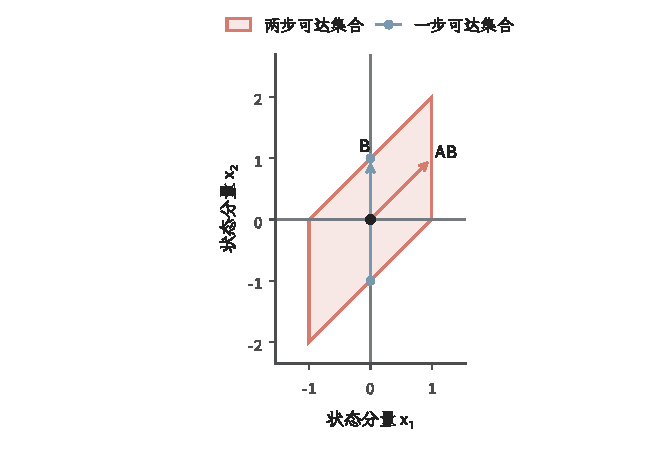
\includegraphics[width=\linewidth]{figures/01-mathematical-preliminaries/05-dynamical-systems-control-decision-and-games/matplotlib/concepts-dynamics/reachable-directions.pdf}
  \caption{教学系统$\bm A=\left[\begin{smallmatrix}1&1\\0&1\end{smallmatrix}\right]$、
  $\bm B=(0,1)^\top$从零出发。蓝色线段为$|u_0|\leq1$的一步可达集合，
  红色区域为$|u_0|,|u_1|\leq1$的两步可达集合；箭头为$\bm B$与$\bm A\bm B$。
  幅值限制用于显示可达区域，不属于无约束可控性秩判据的假设。}
  \label{fig:control-reachable-directions}
\end{figure}

连续时间系统$\dot{\bm x}_t=\bm A\bm x_t+\bm B\bm u_t$在固定$T>0$上的终态为
\[
  \bm x_T=e^{\bm A T}\bm x_0+
  \int_0^T e^{\bm A(T-s)}\bm B\bm u_s\,\mathrm ds.
\]
这里允许$\bm u\in L^2([0,T];\mathbb R^m)$，不加幅值限制。
输入通过积分累积，对应的\term{可控Gram矩阵}（controllability Gramian）为
\begin{equation}
  \bm W_{\mathrm c}(T)=
  \int_0^T e^{\bm A s}\bm B\bm B^\top e^{\bm A^\top s}\,\mathrm ds.
  \label{eq:control-controllability-gramian}
\end{equation}
系统在$[0,T]$可控当且仅当$\bm W_{\mathrm c}(T)\succ\bm0$。
证明先说明奇异矩阵为什么留下不可达方向，再为正定矩阵构造到达任意目标的输入。
为此计算
\[
  \bm q^\top\bm W_{\mathrm c}(T)\bm q
  =\int_0^T\|\bm B^\top e^{\bm A^\top s}\bm q\|_2^2\,\mathrm ds.
\]
若矩阵奇异，某个非零$\bm q$使连续的非负被积函数恒为零，于是该方向与全部受控
终态增量正交。若矩阵正定，对$\bm d=\bm x_{\mathrm f}-e^{\bm A T}\bm x_0$取
\[
  \bm u_s=\bm B^\top e^{\bm A^\top(T-s)}\bm W_{\mathrm c}(T)^{-1}\bm d,
\]
代回便得到终态增量$\bm d$。被积函数恒为零使
$\bm B^\top e^{\bm A^\top s}\bm q$恒为零；
对这个向量函数在$s=0$逐阶求导，得到$\bm q^\top\bm A^k\bm B=0$。
反向由矩阵指数级数成立；再结合Cayley--Hamilton定理，
可知连续系统同样由式~\eqref{eq:control-controllability-matrix}判定。
离散情形的对应Gram矩阵为
$\sum_{j=0}^{N-1}\bm A^j\bm B\bm B^\top(\bm A^\top)^j$。
这些结论依赖线性结构，不能用一点的线性化代替非线性系统的全局可控性。

若只想定位哪个模式不受输入影响，可以直接检查左特征向量。
\begin{theorem}[Popov--Belevitch--Hautus（PBH）可控性判据]
\label{thm:control-pbh-controllability}
矩阵对$(\bm A,\bm B)$可控，当且仅当对每个复特征值$\lambda\in\sigma(\bm A)$，
\begin{equation}
  \operatorname{rank}[\lambda\bm I-\bm A\ \bm B]=n.
  \label{eq:control-pbh-controllability}
\end{equation}
等价地，不存在非零左特征向量$\bm q^\ast$同时满足
$\bm q^\ast\bm A=\lambda\bm q^\ast$和$\bm q^\ast\bm B=\bm0$。
\end{theorem}
\begin{proof}
若存在这样的向量，则
$\bm q^\ast\bm A^k\bm B=\lambda^k\bm q^\ast\bm B=\bm0$对所有$k\geq0$成立，
所以可控性矩阵不可能满行秩。
反之，其列空间$\bm R_{\mathrm{reach}}$若不满维，便是一个真$\bm A$不变子空间。
正交补$\bm R_{\mathrm{reach}}^{\perp}$在$\bm A^\ast$下不变。在复数域上，
这个非零有限维不变子空间包含$\bm A^\ast$的一个特征向量$\bm q$。
它正交于$\bm B$的每一列，因此对应的左特征向量满足
$\bm q^\ast\bm B=\bm0$，PBH矩阵在相应特征值处不满秩。
\end{proof}

终点可控仍不保证任意指定的中间状态都能实现。给定整条参考$\bm r_t$，
离散系统要求每一步$\bm r_{t+1}-\bm A\bm r_t\in\operatorname{col}(\bm B)$，
并且解出的输入位于允许集合；连续系统则要求参考绝对连续且
$\dot{\bm r}_t-\bm A\bm r_t=\bm B\bm u_t^r$几乎处处成立。
终点可达回答“能否到那里”，而实现整条参考轨迹还要回答“能否按这条路走”。

\subsection{观测条件下的状态可区分性}
已知输入对输出的贡献可以计算并扣除。因此，比较同一输入下的两个初态时，
只需考虑自由响应。为简化记号，下式中的$\bm y_t$表示已经扣除已知输入贡献的输出，
于是前$n$次输出满足
\begin{equation}
  \begin{bmatrix}\bm y_0\\\bm y_1\\\vdots\\\bm y_{n-1}\end{bmatrix}
  =
  \underbrace{\begin{bmatrix}
    \bm C\\\bm C\bm A\\\vdots\\\bm C\bm A^{n-1}
  \end{bmatrix}}_{\mathcal O(\bm C,\bm A)}\bm x_0.
  \label{eq:control-observability-matrix}
\end{equation}
\begin{definition}[可观测性]
\label{def:control-observability-detectability}
若同一已知输入下的输出序列能够区分任意两个不同初态，称$(\bm C,\bm A)$
可观测（observable）。对上述线性时不变系统，这等价于
$\mathcal O(\bm C,\bm A)$满列秩。
\end{definition}

满列秩使式~\eqref{eq:control-observability-matrix}对初态至多有一个解。
反之，若秩不足，存在$\bm v\neq\bm0$满足$\mathcal O\bm v=\bm0$，
初态$\bm x_0$与$\bm x_0+\bm v$的前$n$次输出便相同。
Cayley--Hamilton定理使以后所有$\bm C\bm A^k\bm v$也是前$n$项的线性组合，
延长观测仍无法区分两者。这同时证明了定义中的等价关系。
对可控性PBH判据取转置，得到可观测性条件
\begin{equation}
  \operatorname{rank}\begin{bmatrix}\lambda\bm I-\bm A\\\bm C\end{bmatrix}=n
  \quad\text{对每个 }\lambda\in\sigma(\bm A).
  \label{eq:control-pbh-observability}
\end{equation}
连续时间在任意固定正时长、无噪声的完整输出上也有相同秩条件；
等价的观测Gram矩阵是
$\int_0^T e^{\bm A^\top s}\bm C^\top\bm C e^{\bm A s}\,\mathrm ds$。

温度模型的$C=1$使无噪声当前读数就能区分状态。有噪声时，同一个读数可能来自
多个状态，结构可观测性并不提供单次误差上界。
第~\ref{sec:dynamical-state-space-filtering}节建立的预测、滤波和平滑还需初态分布与
噪声规律才能计算估计精度。本章接下来使用较弱的可检测条件，判断哪些看不见的误差
仍能自行衰减，而不要求把所有状态都精确恢复。

\section{策略的轨迹收敛与稳定}
\label{sec:control-closed-loop-stability}

可控性判断输入的结构能力，稳定性判断所选反馈实际产生的长期行为。
第~\ref{sec:dynamical-stability-sensitivity}节已区分平衡点稳定、渐近稳定与指数稳定。
在线性定常系统中，以下“稳定矩阵”统一指离散时间特征值模小于$1$，
或连续时间特征值实部小于$0$；它们都给出齐次系统的指数衰减。
有持续噪声时，所讨论的是齐次初始误差衰减和受迫二阶矩有界，不能称为每条路径趋零。

\subsection{不可控与不可观测模式的稳定条件}
反馈$\bm u=-\bm K\bm x$把状态矩阵改为$\bm A-\bm B\bm K$。
这个矩阵的特征值称为闭环极点（closed-loop poles），它们决定线性齐次响应的衰减或增长。
为了使状态偏差最终消退，只需要通过反馈改变原先不衰减的模式；已经自行
衰减的方向可以保留。这个较弱的要求称为稳定化。
\begin{definition}[可稳定性]
\label{def:control-stabilizability}
若存在$\bm K$使$\bm A-\bm B\bm K$稳定，称矩阵对$(\bm A,\bm B)$
可稳定（stabilizable）。稳定区域按系统采用的离散或连续时间确定。
\end{definition}

从可控性走到固定反馈的存在性，还要用到极点配置定理：对实可控对
$(\bm A_{\mathrm c},\bm B_{\mathrm c})$，任给次数等于其状态维数的实首一多项式，
都存在实增益$\bm K_{\mathrm c}$，使该多项式成为
$\bm A_{\mathrm c}-\bm B_{\mathrm c}\bm K_{\mathrm c}$的特征多项式。
因此可以选择全部根位于单位圆内，或在连续时间选择全部根位于左半平面。
这里引用这一标准存在定理；它不是仅由“有限时间可以到达任意终点”一句话直接推出的结论\scite{math-khalil2002nonlinear}

在前面的二维传播例中，取
$\bm A=\left[\begin{smallmatrix}1&1\\0&1\end{smallmatrix}\right]$、
$\bm B=(0,1)^\top$和$\bm K=(k_1,k_2)$，可直接算得
\[
 \det(\lambda\bm I-\bm A+\bm B\bm K)
 =\lambda^2+(k_2-2)\lambda+1-k_2+k_1.
\]
希望闭环根为$0.2,0.5$时，将系数与
$(\lambda-0.2)(\lambda-0.5)=\lambda^2-0.7\lambda+0.1$比较，
得到$k_2=1.3,k_1=0.4$。这个例子展示怎样用固定增益安排谱，而不再逐时刻另选输入序列。

令$\bm R_{\mathrm{reach}}$为可控性矩阵的列空间，选取以其一组基为前若干列的可逆矩阵$\bm T$。
由于$\bm A\bm R_{\mathrm{reach}}\subseteq\bm R_{\mathrm{reach}}$且
$\operatorname{col}(\bm B)\subseteq\bm R_{\mathrm{reach}}$，坐标$\bm z_t=\bm T^{-1}\bm x_t$给出
\[
  \bm T^{-1}\bm A\bm T=
  \begin{bmatrix}\bm A_{\mathrm c}&\bm A_{1,2}\\
                  \bm0&\bm A_{\mathrm{uc}}\end{bmatrix},
  \qquad
  \bm T^{-1}\bm B=\begin{bmatrix}\bm B_{\mathrm c}\\\bm0\end{bmatrix},
\]
其中$(\bm A_{\mathrm c},\bm B_{\mathrm c})$可控。这是可控分解：上块接收输入，
下块只能自行演化。把$\bm K\bm T$写成$[\bm K_{\mathrm c}\ \bm K_{\mathrm{uc}}]$，
闭环矩阵成为
\[
  \begin{bmatrix}
    \bm A_{\mathrm c}-\bm B_{\mathrm c}\bm K_{\mathrm c}
      &\bm A_{1,2}-\bm B_{\mathrm c}\bm K_{\mathrm{uc}}\\
    \bm0&\bm A_{\mathrm{uc}}
  \end{bmatrix}.
\]
可控块可以用极点配置选择稳定特征值，不可控块的特征值却不受反馈影响。
因此可稳定当且仅当不可控块本身稳定，PBH形式为
\begin{equation}
  \operatorname{rank}[\lambda\bm I-\bm A\ \bm B]=n
  \quad\text{对每个 }|\lambda|\geq1.
  \label{eq:control-pbh-stabilizability}
\end{equation}
只需检查$\bm A$的特征值，其余$\lambda$自动满足秩条件；
连续时间把$|\lambda|\geq1$换成$\operatorname{Re}\lambda\geq0$。

\begin{example}[不可控但可稳定的系统]
\label{ex:control-stabilizable-not-controllable}
取
\[
  \bm A=\begin{bmatrix}1.2&0\\0&0.5\end{bmatrix},
  \qquad \bm B=\begin{bmatrix}1\\0\end{bmatrix}.
\]
可控性矩阵$[\bm B\ \bm A\bm B]
=\left[\begin{smallmatrix}1&1.2\\0&0\end{smallmatrix}\right]$仅有秩$1$。
第二个模式不可控，但其特征值$0.5$已经稳定。取$\bm K=(1,0)$，
闭环特征值为$0.2,0.5$，所以系统可稳定。若交换$\bm B$的两个分量，
输入只能作用到$0.5$模式，$1.2$模式不可控，系统便不可稳定。
\end{example}

传感器一侧有对应的问题：无法识别的初始误差，能否不经校正就逐渐消失？
\begin{definition}[可检测性]
\label{def:control-detectability}
若存在$\bm L$使$\bm A-\bm L\bm C$稳定，称$(\bm C,\bm A)$
可检测（detectable）。
\end{definition}
它不要求每个初态都可恢复，只要求不可观测的模式自行稳定。其离散PBH条件为
\begin{equation}
  \operatorname{rank}
  \begin{bmatrix}\lambda\bm I-\bm A\\\bm C\end{bmatrix}=n
  \quad\text{对每个 }|\lambda|\geq1.
  \label{eq:control-pbh-detectability}
\end{equation}
这一等价关系来自转置对偶：$(\bm A^\top,\bm C^\top)$的可控性矩阵的转置，
正是$(\bm C,\bm A)$的观测矩阵。对前者作可控分解，其不可控块对应原系统的
不可观测模式，又有
$\bm A^\top-\bm C^\top\bm L^\top=(\bm A-\bm L\bm C)^\top$。
因此，不可观测块稳定时可配置其余误差模式；存在不可观测的非衰减模式时，
任何$\bm L$都无法移动它。连续时间同样用闭右半平面替换单位圆外。

继续取示例~\ref{ex:control-stabilizable-not-controllable}的$\bm A$。
$\bm C=(1,0)$看得见$1.2$模式，看不见会自行衰减的$0.5$模式，所以不可观测却可检测。
改用$\bm C=(0,1)$便看不到危险模式，任何估计器的确定性初始误差都不能依靠输出
把该方向统一消除。表~\ref{tab:control-structural-properties}汇总四种条件；
输入或观测能否影响全部方向，与是否足以保证长期稳定，是不同的要求。
\begin{table*}[htbp]
  \centering
  \begin{tabularx}{\linewidth}{lXXX}
    \toprule
    性质 & 所比较的对象 & 哪些方向必须处理 & 二维例的判断\\
    \midrule
    可控 & 输入与终态 & 全部状态方向 & 否，输入无法改变第二坐标\\
    可稳定 & 反馈与闭环谱 & 不稳定及临界模式 & 是，$1.2$模式受控\\
    可观测 & 初态与输出序列 & 全部状态方向 & 否，输出不含第二坐标\\
    可检测 & 观测器与误差谱 & 不稳定及临界模式 & 是，$1.2$模式可见\\
    \bottomrule
  \end{tabularx}
  \caption{固定$\bm A=\operatorname{diag}(1.2,0.5)$、
  $\bm B=(1,0)^\top$、$\bm C=(1,0)$比较四种结构条件。
  第二模式虽不可控、不可观测，却自行衰减；若把其特征值改为$1.1$，
  可稳定与可检测也会失败。连续时间按实部判断危险模式。}
  \label{tab:control-structural-properties}
  \label{tab:control-structural-comparison}
\end{table*}

\subsection{状态反馈下的闭环稳定}
\label{sec:control-state-feedback-stability}
结构条件允许稳定化以后，仍需选定反馈并检查实际闭环。线性状态反馈给出
\begin{equation}
  \bm u_t=-\bm K\bm x_t,
  \qquad \bm x_{t+1}=(\bm A-\bm B\bm K)\bm x_t.
  \label{eq:control-state-feedback}
\end{equation}
负号只是增益约定。按定理~\ref{thm:dynamical-discrete-spectral-stability}，
闭环渐近稳定当且仅当$\rho(\bm A-\bm B\bm K)<1$。
也可以按定理~\ref{thm:dynamical-discrete-lyapunov-equation}找$\bm P\succ\bm0$，
使$\bm P-\bm F^\top\bm P\bm F\succ\bm0$，其中$\bm F=\bm A-\bm B\bm K$。
连续时间则检查$\bm F$的特征值实部或
$\bm F^\top\bm P+\bm P\bm F\prec\bm0$。

不同稳定增益并不产生同样的响应。在无约束、无噪声的温度模型中先以零为目标，
取$u_t=-kx_t$，有$x_t=(0.8-k)^t x_0$。增益$k=0.3$使系数为$0.5$，
$k=0.7$使系数为$0.1$；对相同初态，后者每步收缩更多，却把初始输入幅值
从$0.3|x_0|$提高到$0.7|x_0|$。取$k=1.4$则得到$-0.6$，
状态交替过零，收敛反而比$0.5$慢。稳定范围是$-0.2<k<1.8$，
不是增益越大越快；有饱和时这些线性计算也不再直接适用。

多维系统还要区分渐近速度与瞬态放大。比较
\[
  \bm F_1=0.5\bm I,\qquad
  \bm F_2=\begin{bmatrix}0.5&4\\0&0.5\end{bmatrix}.
\]
二者特征值均为$0.5$，但从$(0,1)^\top$出发，第一步的状态范数分别为
$0.5$和$\sqrt{16.25}>4$。事实上
\[
  \bm F_2^t=
  \begin{bmatrix}0.5^t&4t\,0.5^{t-1}\\0&0.5^t\end{bmatrix}
  \quad(t\geq1).
\]
非对角耦合先放大误差，随后才被指数衰减压低。两者都可以在$\bm A=\bm B=\bm I$
的系统中由$\bm K_i=\bm I-\bm F_i$实现，第二种增益也引入较强的交叉输入。
因此评价反馈时应共同看$\|\bm F^t\|_2$、输入$\|\bm K\bm x_t\|_2$与长期衰减，
而不是仅比较最大特征值。二次成本在下一小节把状态偏差与输入幅值纳入同一准则，
但“稳定”本身并没有选定这一偏好。

非线性系统无法靠一个常矩阵描述全部区域。此时可以先找一个衡量偏离程度的函数，
再选动作让它下降，这就是控制Lyapunov方法。
\begin{definition}[控制Lyapunov函数条件]
\label{def:control-clf}
考虑$\dot{\bm x}_t=\bm f(\bm x_t)+\bm G(\bm x_t)\bm u_t$，目标为原点，
输入属于$U$。若某邻域内的$C^1$函数$V$满足$V(\bm0)=0$、
$V(\bm x)>0$（$\bm x\neq\bm0$），且有正定连续函数$W$使
\[
  \inf_{\bm u\in U}
  \nabla V(\bm x)^\top(\bm f(\bm x)+\bm G(\bm x)\bm u)
  \leq-W(\bm x),
\]
称$V$提供一个\term{控制Lyapunov函数}（control Lyapunov function, CLF）条件：
每个非零状态至少应能选择一个使偏离量严格下降的动作。
调用反馈稳定性结论时，还要求下降动作确实可取到。
\end{definition}

点态存在动作不等于已经构造出适定反馈。若能选出局部Lipschitz反馈$\kappa$，
使原点为平衡、且沿闭环$\dot V\leq-W$，即可回用
定理~\ref{thm:dynamical-nonlinear-lyapunov}得到局部渐近稳定。
若进一步有$c_1\|\bm x\|_2^2\leq V\leq c_2\|\bm x\|_2^2$和
$W\geq c_3\|\bm x\|_2^2$，便有
$V_t\leq e^{-c_3t/c_2}V_0$；全局结论还需全域条件与解的延拓。
例如$\dot x_t=x_t^3+u_t$取$V(x)=x^2/2$、$u_t=-x_t^3-kx_t$（$k>0$），
得到$\dot V=-kx_t^2$和$x_t=e^{-kt}x_0$。这个反馈在无界输入下成立；
若$|u_t|\leq u_{\max}$，大状态处抵消$x_t^3$所需的动作可能不可行，
只能在经过核验的区域中声明稳定\scite{math-khalil2002nonlinear}

\subsection{二次反馈下的稳定化解}
\label{sec:control-lqr-riccati}
要在减小状态偏差与限制输入幅值之间作出具体选择，可以分别给两者加上二次代价。
这一特例能够通过逐步配方直接算出反馈，无须先掌握一般价值优化理论。
\begin{definition}[有限时域线性二次调节]
\label{def:control-finite-horizon-lqr}
考虑状态完全可见的系统
\begin{equation}
  \bm x_{t+1}=\bm A\bm x_t+\bm B\bm u_t+\bm w_{t+1},
  \qquad t=0,\ldots,T-1,
  \label{eq:control-lqr-dynamics}
\end{equation}
以及风险中性的期望成本
\begin{equation}
  J=\mathbb E\left[
  \bm x_T^\top\bm Q_T\bm x_T+
  \sum_{t=0}^{T-1}
  (\bm x_t^\top\bm Q\bm x_t+\bm u_t^\top\bm R\bm u_t)\right].
  \label{eq:control-lqr-cost}
\end{equation}
其中$\bm Q,\bm Q_T\succeq\bm0$为$n\times n$对称矩阵，
$\bm R\succ\bm0$为$m\times m$对称矩阵。输入无幅值限制。
在非预见的状态反馈策略中最小化$J$，称为\term{线性二次调节}
（linear-quadratic regulation, LQR）。
\end{definition}

本小节的$\bm w_t$服从固定但不必高斯的分布，均值为零，协方差为
$\bm\Sigma_{\mathrm w}$，各时刻独立并独立于初态；初态二阶矩有限。
动作对截至$t$的状态历史$\mathcal F_t=\sigma(\bm x_0,\ldots,\bm x_t)$可测，
因而$\bm w_{t+1}$独立于当前状态和动作。状态代价半正定允许某些方向不直接计价，
控制代价正定保证每一步动作最小化严格凸。

用$\Pi_t$表示从$t$到$T-1$、适应上述状态信息的允许策略，
以$\mathbb E_{t,\bm x}$表示从时刻$t$的状态$\bm x$开始运行所得的期望。
最优剩余成本定义为
\[
  \begin{aligned}
  V_t(\bm x)=\inf_{\pi\in\Pi_t}\mathbb E_{t,\bm x}\biggl[
    &\bm x_T^\top\bm Q_T\bm x_T\\
    &+\sum_{\tau=t}^{T-1}
      (\bm x_\tau^\top\bm Q\bm x_\tau+
       \bm u_\tau^\top\bm R\bm u_\tau)\biggr].
  \end{aligned}
\]
这里的下确界取遍反馈策略而不是预先固定的动作序列；
终端为$V_T(\bm x)=\bm x^\top\bm Q_T\bm x$。
将当前阶段与未来分开，条件期望的迭代性质给出
\begin{equation}
  \begin{aligned}
  V_t(\bm x)=\min_{\bm u}\bigl\{&
    \bm x^\top\bm Q\bm x+\bm u^\top\bm R\bm u\\
    &+\mathbb E[V_{t+1}(\bm A\bm x+\bm B\bm u+\bm w_{t+1})]\bigr\}.
  \end{aligned}
  \label{eq:control-lqr-bellman}
\end{equation}
对任意策略，后续成本至少为下一状态的$V_{t+1}$；若下一步的下界可由反馈取得，
先选当前极小动作，再接上该反馈，就取得等号。下面的反向归纳同时构造这些可取到的
动作，因此这里不依赖尚未证明的一般最优策略存在性。这一递推的通用形式将在
第~\ref{chap:decision-theory-and-dynamic-risk}章展开\scite{math-anderson2007lqr}

\begin{theorem}[有限时域LQR与Riccati递推]
\label{thm:control-finite-horizon-lqr}
在上述条件下，
$V_t(\bm x)=\bm x^\top\bm P_t\bm x+c_t$，
其中$\bm P_T=\bm Q_T$、$c_T=0$。令
\begin{equation}
  \begin{aligned}
    \bm S_t&=\bm R+\bm B^\top\bm P_{t+1}\bm B,\\
    \bm K_t&=\bm S_t^{-1}\bm B^\top\bm P_{t+1}\bm A,
  \end{aligned}
  \label{eq:control-lqr-gain}
\end{equation}
则最优动作是$\bm u_t^\ast=-\bm K_t\bm x_t$，矩阵满足
\begin{equation}
  \begin{aligned}
  \bm P_t={}&\bm Q+\bm A^\top\bm P_{t+1}\bm A\\
       &-\bm A^\top\bm P_{t+1}\bm B\bm S_t^{-1}
                    \bm B^\top\bm P_{t+1}\bm A,
  \end{aligned}
  \label{eq:control-discrete-riccati-recursion}
\end{equation}
噪声只进入常数项
\begin{equation}
  c_t=c_{t+1}+\operatorname{tr}(\bm P_{t+1}\bm\Sigma_{\mathrm w}).
  \label{eq:control-lqr-noise-constant}
\end{equation}
\end{theorem}
\begin{proof}
在终端结论成立。假设$t+1$时刻的表达和最优反馈已构造，
记$\bm z=\bm A\bm x+\bm B\bm u$。噪声的零均值、协方差与独立性给出
\[
  \mathbb E[V_{t+1}(\bm z+\bm w_{t+1})]
  =\bm z^\top\bm P_{t+1}\bm z+
    \operatorname{tr}(\bm P_{t+1}\bm\Sigma_{\mathrm w})+c_{t+1}.
\]
交叉项条件期望为零。将$\bm z$展开，当前目标为
\begin{align*}
  &\bm x^\top(\bm Q+\bm A^\top\bm P_{t+1}\bm A)\bm x
   +2\bm u^\top\bm B^\top\bm P_{t+1}\bm A\bm x
   +\bm u^\top\bm S_t\bm u\\
  &\qquad+\operatorname{tr}(\bm P_{t+1}\bm\Sigma_{\mathrm w})+c_{t+1}.
\end{align*}
由$\bm P_{t+1}\succeq\bm0$、$\bm R\succ\bm0$得$\bm S_t\succ\bm0$。
动作相关项可以完整配方：
\begin{align*}
  &\bm u^\top\bm S_t\bm u+
       2\bm u^\top\bm B^\top\bm P_{t+1}\bm A\bm x\\
  &\quad=(\bm u+\bm K_t\bm x)^\top\bm S_t(\bm u+\bm K_t\bm x)
       -\bm x^\top\bm K_t^\top\bm S_t\bm K_t\bm x.
\end{align*}
平方项非负且仅在$\bm u=-\bm K_t\bm x$处为零。合并剩余二次项与常数项，
分别得到式~\eqref{eq:control-discrete-riccati-recursion}和
式~\eqref{eq:control-lqr-noise-constant}。所得二次型也是
\[
  \bm x^\top\bm P_t\bm x
  =\min_{\bm u}\{
   \bm x^\top\bm Q\bm x+\bm u^\top\bm R\bm u+
   (\bm A\bm x+\bm B\bm u)^\top\bm P_{t+1}(\bm A\bm x+\bm B\bm u)\},
\]
故$\bm P_t\succeq\bm0$，归纳可以继续。线性极小动作可测，并在有限时域保持二阶矩
有限；将这些动作依次拼接，取得每一步下界，证明最优值确实可达。
\end{proof}

线性动态把二次型变为状态与动作的联合二次型，动作配方后又留下状态二次型。
这解释了Riccati构造为何在本模型中闭合，也说明不能把非线性动态随意换成Jacobian
就声称得到了原问题的精确解。
噪声只影响常数项同样有边界：非零均值通常产生线性项和仿射偏置；
噪声分布随动作或状态变化时，增益也可能变化；若目标更加重视成本很大的
少数结果，即后文的尾部风险，原增益同样未必最优。
若权重和噪声协方差是预先给定的逐时量，只需在第$t$步分别用
$\bm Q_t,\bm R_t,\bm\Sigma_{\mathrm w,t+1}$替换对应矩阵，
保持$\bm Q_t\succeq\bm0,\bm R_t\succ\bm0$和独立零均值条件，同一反向归纳仍成立。

为了看清有限时域的成本最优为何未必保证长期稳定，下面把温度模型的衰减系数
$0.8$改为增长系数$1.2$，考察无输入时会放大状态的标量系统。
取$x_{t+1}=1.2x_t+u_t$、$Q=R=1$且无噪声。记下一步系数为$p=P_{t+1}$，
当前目标的配方为
\[
  \begin{aligned}
  x^2+u^2+p(1.2x+u)^2
   ={}&(1+p)\left(u+\frac{1.2p}{1+p}x\right)^2\\
     &+\left(1+1.44p-\frac{1.44p^2}{1+p}\right)x^2.
  \end{aligned}
\]
因此
\[
  S_t=1+P_{t+1},\qquad
  K_t=\frac{1.2P_{t+1}}{1+P_{t+1}},
  \qquad
  P_t=1+\frac{1.44P_{t+1}}{1+P_{t+1}}.
\]
若$P_T=0$，则$P_{T-1}=1,K_{T-1}=0$；
最后一个动作之后没有状态代价，故此时不用力。
再向前一步有$P_{T-2}=1.72,K_{T-2}=0.6$。
有限时域的最优反馈未必在每一步都使闭环矩阵稳定，$K_{T-1}=0$就是反例。
所以有限时域内能够通过配方求出最优动作，并不能证明无限时域内存在稳定的
最优反馈。

为处理长期稳定化，现切换到确定性、时不变、无折扣系统，即
$\bm w_{t+1}=\bm0$，目标为
\[
  J_\infty=\sum_{t=0}^\infty
  (\bm x_t^\top\bm Q\bm x_t+\bm u_t^\top\bm R\bm u_t).
\]
若反馈与二次系数不再随时间变化，递推给出
\term{离散代数Riccati方程}（discrete algebraic Riccati equation, DARE）：
\begin{equation}
  \begin{aligned}
  \bm P={}&\bm Q+\bm A^\top\bm P\bm A\\
     &-\bm A^\top\bm P\bm B
       (\bm R+\bm B^\top\bm P\bm B)^{-1}\bm B^\top\bm P\bm A.
  \end{aligned}
  \label{eq:control-dare}
\end{equation}
所需的\term{稳定化解}（stabilizing solution）不仅满足$\bm P\succeq\bm0$，
还要求其增益
$\bm K=(\bm R+\bm B^\top\bm P\bm B)^{-1}\bm B^\top\bm P\bm A$
使闭环稳定。

\begin{theorem}[无限时域LQR的稳定化解]
\label{thm:control-infinite-horizon-lqr}
设$\bm Q\succeq\bm0$、$\bm R\succ\bm0$，
$(\bm A,\bm B)$可稳定且$(\bm Q^{1/2},\bm A)$可检测。
则式~\eqref{eq:control-dare}存在唯一半正定稳定化解$\bm P$。
相应反馈使闭环渐近稳定，并在所有允许控制序列中给出无折扣二次总成本的
最优值$V(\bm x)=\bm x^\top\bm P\bm x$。
\end{theorem}
\begin{proof}
取长度$N$、终端代价为零的有限问题，记其初始价值矩阵为$\bm P^{(N)}$。
增加一个非负阶段成本不能降低最优成本，故
$\bm0\preceq\bm P^{(N)}\preceq\bm P^{(N+1)}$。
可稳定性提供$\overline{\bm K}$使
$\overline{\bm F}=\bm A-\bm B\overline{\bm K}$稳定。始终用此反馈的成本矩阵为
\[
  \overline{\bm P}=\sum_{j=0}^\infty
  (\overline{\bm F}^\top)^j
  (\bm Q+\overline{\bm K}^\top\bm R\overline{\bm K})
  \overline{\bm F}^j,
\]
级数由指数衰减收敛，且$\bm P^{(N)}\preceq\overline{\bm P}$。
每个二次型$\bm x^\top\bm P^{(N)}\bm x$单调有界，
再用极化恒等式恢复矩阵各元素，得到$\bm P^{(N)}\to\bm P\succeq\bm0$。
Riccati映射连续，因为待逆矩阵始终不小于$\bm R\succ\bm0$；
对$\bm P^{(N+1)}=\mathcal R(\bm P^{(N)})$取极限得到DARE。

令$\bm F=\bm A-\bm B\bm K$，DARE按增益改写为
\begin{equation}
  \bm P-\bm F^\top\bm P\bm F=\bm Q+\bm K^\top\bm R\bm K.
  \label{eq:control-dare-lyapunov}
\end{equation}
若$\bm F\bm z=\lambda\bm z$且$\bm z\neq\bm0,|\lambda|\geq1$，
在两侧乘$\bm z^\ast,\bm z$得到
\[
  (1-|\lambda|^2)\bm z^\ast\bm P\bm z
  =\|\bm Q^{1/2}\bm z\|_2^2+\|\bm R^{1/2}\bm K\bm z\|_2^2.
\]
左侧非正，右侧非负，所以均为零，特别有
$\bm Q^{1/2}\bm z=\bm0,\bm K\bm z=\bm0$。
于是$\bm A\bm z=(\bm F+\bm B\bm K)\bm z=\lambda\bm z$，
违反$(\bm Q^{1/2},\bm A)$的可检测性。因此$\bm F$稳定。

存在且稳定还不足以完成最优性证明。记$\bm S=\bm R+\bm B^\top\bm P\bm B$，
对任意控制沿前$N$步累加配方恒等式：
\begin{align*}
  &\sum_{t=0}^{N-1}
    (\bm x_t^\top\bm Q\bm x_t+\bm u_t^\top\bm R\bm u_t)
    +\bm x_N^\top\bm P\bm x_N\\
  &\quad=\bm x_0^\top\bm P\bm x_0+
    \sum_{t=0}^{N-1}
    (\bm u_t+\bm K\bm x_t)^\top\bm S(\bm u_t+\bm K\bm x_t).
\end{align*}
不能直接丢弃左侧终端项。若该控制的总成本有限，非负级数的项趋零，给出
$\bm Q^{1/2}\bm x_t\to\bm0$及$\bm u_t\to\bm0$，后者使用$\bm R\succ\bm0$。
可检测性提供$\bm L$使$\bm H=\bm A-\bm L\bm Q^{1/2}$稳定，于是
\[
  \bm x_{t+1}=\bm H\bm x_t+
       \underbrace{\bm B\bm u_t+\bm L\bm Q^{1/2}\bm x_t}_{\bm d_t\to\bm0}.
\]
展开为$\bm H^t\bm x_0+\sum_{j=0}^{t-1}\bm H^{t-1-j}\bm d_j$。
有限个早期输入的贡献随$t$衰减；晚期输入任意小，且
$\sum_{j\geq0}\|\bm H^j\|_2<\infty$，故卷积尾部也趋零。
因此$\bm x_t\to\bm0$，终端项趋零。

令$N\to\infty$，任何有限成本控制的成本都是
$\bm x_0^\top\bm P\bm x_0$加上一串非负平方项。
采用$\bm u_t=-\bm K\bm x_t$时平方项全为零，闭环稳定保证终端项趋零和总成本有限，
故达到下界；无限成本控制自然不能优于它。
若另有半正定稳定化解，同一配方和终端项论证也使它表示全部初态上的同一个最优成本。
两个对称矩阵的二次型处处相等，矩阵便相等，唯一性得证。
\end{proof}

在前述$A=1.2,B=1,Q=R=1$例中，
\[
  P=1+\frac{1.44P}{1+P},
  \qquad P^2-1.44P-1=0,
\]
半正定根与反馈为
\[
  P=\frac{1.44+\sqrt{6.0736}}2\approx1.952,
  \quad K=\frac{1.2P}{1+P}\approx0.794,
  \quad 1.2-K\approx0.406.
\]
另一个根为负，不表示非负总成本。
可检测条件中的“输出”是成本所见的$\bm Q^{1/2}\bm x$，不是传感器的$\bm C\bm x$；
两种可检测条件不能替换。

若$A=1.2,B=1,Q=0,R=1$，系统可控却不满足成本可检测性。
DARE有$P=0$与$P=0.44$两个半正定根。前者给$K=0$和不稳定闭环$1.2$，
后者给稳定闭环$5/6$。原目标只惩罚控制，$u_t=0$以零成本全局最优，
稳定化反馈反而支付正成本。这个反例说明稳定化与成本最优之间的联系确实依赖假设。
若恢复持续非零加性噪声，稳定闭环通常有非零稳态协方差，单步期望成本不趋零，
无折扣总期望成本通常发散；除噪声传播恰好不被成本计价等退化情形，
应改用有限、折扣或长期平均成本，而不是沿用本定理的确定性总成本。

连续时间也可以直接用代数方程构造稳定反馈，无须先推导有限时域价值。
对$\dot{\bm x}_t=\bm A\bm x_t+\bm B\bm u_t$，连续代数Riccati方程
（continuous algebraic Riccati equation, CARE）为
\begin{equation}
  \bm0=\bm Q+\bm A^\top\bm P+\bm P\bm A
       -\bm P\bm B\bm R^{-1}\bm B^\top\bm P.
  \label{eq:control-care}
\end{equation}
当$\bm Q\succeq\bm0,\bm R\succ\bm0$，且连续时间意义下
$(\bm A,\bm B)$可稳定、$(\bm Q^{1/2},\bm A)$可检测时，CARE有唯一半正定
稳定化解；这是连续线性二次控制的标准代数结论\scite{math-anderson2007lqr}
本处使用其存在性，具体闭环性质还可直接核验。
令$\bm K=\bm R^{-1}\bm B^\top\bm P$、$\bm F=\bm A-\bm B\bm K$，则
\[
  \bm F^\top\bm P+\bm P\bm F=-(\bm Q+\bm K^\top\bm R\bm K).
\]
若$\bm F\bm z=\lambda\bm z$且$\operatorname{Re}\lambda\geq0$，
两侧二次型给出
$2\operatorname{Re}\lambda\,\bm z^\ast\bm P\bm z
=-\|\bm Q^{1/2}\bm z\|_2^2-\|\bm R^{1/2}\bm K\bm z\|_2^2$。
同样推出$\bm Q^{1/2}\bm z=\bm K\bm z=\bm0$，与可检测性矛盾。
所以闭环谱位于左半平面；即使$\bm P$仅半正定，仍可由谱结论另解正定Lyapunov方程。
连续有限时域微分Riccati及价值最优性在
第~\ref{chap:decision-theory-and-dynamic-risk}章主讲；本处的稳定核验不以它们为前提。

\subsection{输出反馈下的估计与闭环稳定}
\label{sec:control-output-feedback-stability}
前面的反馈把真实状态直接写入动作公式。若控制器只有传感器读数，就需要说明
怎样结合模型与读数形成状态估计，以及使用哪一时刻的估计计算动作。
\term{Luenberger观测器}（Luenberger observer）采用
\begin{equation}
  \widehat{\bm x}_{t+1}
  =\bm A\widehat{\bm x}_t+\bm B\bm u_t+
    \bm L(\bm y_t-\bm C\widehat{\bm x}_t).
  \label{eq:control-luenberger-observer}
\end{equation}
无噪声时，误差$\bm e_t^{\mathrm o}=\bm x_t-\widehat{\bm x}_t$满足
$\bm e_{t+1}^{\mathrm o}=(\bm A-\bm L\bm C)\bm e_t^{\mathrm o}$。
可检测性恰好允许选出误差衰减的$\bm L$。
若使用$\bm u_t=-\bm K\widehat{\bm x}_t$，联合系统为
\begin{equation}
  \begin{bmatrix}\bm x_{t+1}\\\bm e_{t+1}^{\mathrm o}\end{bmatrix}
  =
  \begin{bmatrix}
    \bm A-\bm B\bm K&\bm B\bm K\\
    \bm0&\bm A-\bm L\bm C
  \end{bmatrix}
  \begin{bmatrix}\bm x_t\\\bm e_t^{\mathrm o}\end{bmatrix}.
  \label{eq:control-separation-block}
\end{equation}
这个\term{分离原理}（separation principle）说的是闭环谱可以分开设计：
特征行列式等于两个对角块特征行列式之积，故联合谱恰为二者的并集。
当两块都稳定时，联合矩阵稳定；反过来，任一块的危险特征值也保留在联合谱中。
因而确定性观测器与状态反馈可以分别作稳定设计；这一论证并未涉及成本最优。

有噪声时，还需区分预测协方差与观测更新后的协方差。
在式~\eqref{eq:control-lqr-dynamics}及
$\bm y_t=\bm C\bm x_t+\bm v_t$中，令$\bm w_t,\bm v_t$分别为独立同分布零均值
噪声，协方差为$\bm\Sigma_{\mathrm w}\succeq\bm0,\bm\Sigma_{\mathrm v}\succ\bm0$，
两族与初态相互独立，初态二阶矩有限，估计器从先验均值及协方差初始化。
若要将Kalman估计解释为精确条件均值，再要求初态和噪声联合高斯；
非高斯时以下递推仍描述相应线性滤波器的误差矩，不自动描述完整后验。

以$\bm\Pi_t$记看到$\bm y_t$之前的预测误差协方差。高斯情形下，
$\widehat{\bm x}_{t|t-1}$是给定截至$t-1$的观测及已执行控制后的条件均值。
在初始时刻，$\bm\Pi_0$由尚未使用$y_0$的先验给出。
更新增益$\bm M_t$与合并预测增益$\bm L_t$分别为
\[
  \bm M_t=\bm\Pi_t\bm C^\top
       (\bm C\bm\Pi_t\bm C^\top+\bm\Sigma_{\mathrm v})^{-1},
  \qquad \bm L_t=\bm A\bm M_t.
\]
先更新再预测，可以写成
\[
  \widehat{\bm x}_{t+1|t}
  =\bm A\widehat{\bm x}_{t|t-1}+\bm B\bm u_t+
       \bm L_t(\bm y_t-\bm C\widehat{\bm x}_{t|t-1}).
\]
所以预测误差的齐次矩阵为$\bm A-\bm L_t\bm C$，不能遗漏增益中的$\bm A$。
稳态预测协方差满足
\begin{equation}
  \begin{aligned}
  \bm\Pi={}&\bm A\bm\Pi\bm A^\top+\bm\Sigma_{\mathrm w}\\
     &-\bm A\bm\Pi\bm C^\top
       (\bm C\bm\Pi\bm C^\top+\bm\Sigma_{\mathrm v})^{-1}
       \bm C\bm\Pi\bm A^\top.
  \end{aligned}
  \label{eq:control-filter-dare}
\end{equation}
控制DARE中作$\bm A\mapsto\bm A^\top,\bm B\mapsto\bm C^\top,
\bm Q\mapsto\bm\Sigma_{\mathrm w},\bm R\mapsto\bm\Sigma_{\mathrm v}$便得到此式。
公式的转置对偶联系的是两个矩阵计算问题，并不使状态成本与估计协方差具有相同含义。

\begin{theorem}[稳态预测滤波的充分条件]
\label{thm:control-steady-filter}
若$(\bm C,\bm A)$可检测、$(\bm A,\bm\Sigma_{\mathrm w}^{1/2})$可稳定，
且$\bm\Sigma_{\mathrm v}\succ\bm0$，则式~\eqref{eq:control-filter-dare}
有唯一半正定稳定化解$\bm\Pi$。从任意有限$\bm\Pi_0\succeq\bm0$出发的
预测协方差递推收敛到$\bm\Pi$，稳态$\bm L=\bm A\bm M$使
$\bm A-\bm L\bm C$稳定。
\end{theorem}
\begin{proof}
对偶代换把本定理的两个结构条件分别变为无限LQR定理的可稳定、可检测条件，
故解的存在、唯一与稳定性成立。为说明一般初始协方差的收敛，记滤波Riccati映射为
$\Phi$。固定任意合并增益$\bm L$，定义
\[
  \Psi_{\bm L}(\bm X)
  =(\bm A-\bm L\bm C)\bm X(\bm A-\bm L\bm C)^\top+
     \bm\Sigma_{\mathrm w}+\bm L\bm\Sigma_{\mathrm v}\bm L^\top.
\]
配方表明$\Phi(\bm X)\preceq\Psi_{\bm L}(\bm X)$，等号在对应Kalman增益处成立。
又若$\bm X\succeq\bm Y$，每个固定增益下
$\Psi_{\bm L}(\bm X)\succeq\Psi_{\bm L}(\bm Y)$；
取$\bm X$的极小增益便得$\Phi(\bm X)\succeq\Phi(\bm Y)$。
取稳态增益$\bm L$，有$\Psi_{\bm L}(\bm\Pi)=\bm\Pi$，并由单调性归纳得到
\[
  \Phi^t(\bm0)\preceq\Phi^t(\bm\Pi_0)
                     \preceq\Psi_{\bm L}^t(\bm\Pi_0).
\]
左端按对偶有限时域构造收敛到$\bm\Pi$；
右端与$\bm\Pi$之差为
$(\bm A-\bm L\bm C)^t(\bm\Pi_0-\bm\Pi)
 [(\bm A-\bm L\bm C)^\top]^t$，也趋零，夹逼得证。
\end{proof}

稳态滤波误差仍由新噪声持续驱动：
\[
  \bm e_{t+1}^{\mathrm p}
  =(\bm A-\bm L\bm C)\bm e_t^{\mathrm p}
     +\bm w_{t+1}-\bm L\bm v_t.
\]
稳定性使初始误差的影响衰减，协方差趋于有限的$\bm\Pi$，
并不使噪声消失。温度例取$\Sigma_{\mathrm w}=0.04,\Sigma_{\mathrm v}=0.09$，
稳态方程为
$\Pi=0.64\Pi+0.04-0.64\Pi^2/(\Pi+0.09)$，
即$\Pi^2-0.0076\Pi-0.0036=0$。正根约为$0.06392$，
$M\approx0.4153,L\approx0.3322$，预测齐次误差系数约为$0.4678$；
稳态预测误差方差为正：即使初始估计误差已消退，新噪声仍会不断造成偏差，
所以不能说每条估计误差路径都趋于零。

实际控制可使用当前观测更新后的$\widehat{\bm x}_{t|t}$。
取$\bm u_t=-\bm K\widehat{\bm x}_{t|t}$，并用预测误差
$\bm e_t^{\mathrm p}=\bm x_t-\widehat{\bm x}_{t|t-1}$，
齐次联合矩阵变为
\[
  \begin{bmatrix}
    \bm A-\bm B\bm K&\bm B\bm K(\bm I-\bm M\bm C)\\
    \bm0&\bm A(\bm I-\bm M\bm C)
  \end{bmatrix}.
\]
附加噪声为
$((\bm w_{t+1}-\bm B\bm K\bm M\bm v_t)^\top,
  (\bm w_{t+1}-\bm A\bm M\bm v_t)^\top)^\top$，
两分量相关，但联合协方差仍有限。
两个对角块稳定时，联合齐次系统稳定；
用幂级数展开协方差，便得有限初始二阶矩下的二阶矩有界和稳态协方差收敛。
非零持续噪声下，状态与预测误差的均值可以趋零，但每次运行仍会受到新噪声扰动，
其样本路径一般不会趋于零。
有限时域线性二次高斯控制的期望成本最优性由
第~\ref{chap:decision-theory-and-dynamic-risk}章另证。
受控观测、输入约束、非线性或模型错设可能改变信息与误差动态，
不能从这里的谱分离直接推出稳定，更不能直接推出最优。

\section{策略的调节与跟踪}
\label{sec:control-regulation-tracking}

前面的反馈围绕原点设计，但温度通常要维持在非零设定值，机械位置也可能要跟随
持续移动的目标。两类任务都能转化为误差系统的稳定问题，区别在于维持目标所需的
输入是常数还是随时间变化。转化前必须先核对目标本身是否符合系统规律。

\subsection{固定目标下的轨迹调节}
\subsubsection{目标平衡与可行输入}
设定值（setpoint）是希望状态或输出最终保持的常数。\term{调节}（regulation）要求偏离
该常数的误差趋于零；它不只要求在某一时刻经过目标。
\begin{definition}[目标平衡与调节误差]
\label{def:control-regulation-equilibrium}
对$\bm x_{t+1}=\bm A\bm x_t+\bm B\bm u_t$，
状态设定值$\bm r$与常值输入$\bm u^r$构成目标平衡，若
\begin{equation}
  (\bm I-\bm A)\bm r=\bm B\bm u^r.
  \label{eq:control-target-equilibrium}
\end{equation}
状态调节误差定义为$\bm e_t=\bm x_t-\bm r$。
若只指定输出设定值$\bm q$，还需寻找平衡状态$\bm r$使
$\bm C\bm r=\bm q$，输出误差为$\bm e_t^y=\bm C\bm x_t-\bm q$。
有输入、状态限制时，目标平衡还须满足$\bm u^r\in U,\bm r\in S$。
\end{definition}

对只指定输出的任务，可解联立方程
\[
  \begin{bmatrix}\bm I-\bm A&-\bm B\\\bm C&\bm0\end{bmatrix}
  \begin{bmatrix}\bm r\\\bm u^r\end{bmatrix}
  =\begin{bmatrix}\bm0\\\bm q\end{bmatrix}.
\]
方程可能无解或有多个解；输出达到设定值也不自动要求所有内部状态相同。
连续时间的平衡条件相应为$\bm A\bm r+\bm B\bm u^r=\bm0$。
这些平衡方程是任务可行性的检查，不是稳定性证明。

\begin{example}[非零温度需要维持输入]
\label{ex:control-temperature-equilibrium}
在无噪声温度模型中，设定值$r=2$要求
$2=0.8\times2+u^r$，所以$u^r=0.4$。
若直接使用$u_t=-0.3(x_t-2)$，在$x_t=2$处输入变成零，
下一步温差便降为$1.6$，因而$2$不是闭环平衡。
若执行器要求$0\leq u\leq1$，单从平衡输入看，
$u^r=0.2r$允许$0\leq r\leq5$；再加状态限制$0\leq x\leq3$，
则目标必须落在$[0,3]$。$r=2,u^r=0.4$满足这两项必要条件。
从某个初态走到目标期间是否也满足约束，还需检查整段闭环轨迹。
\end{example}

\subsubsection{基于误差反馈的轨迹调节}
平衡输入抵消目标位置的自然漂移，反馈只负责消除偏差。对已求得的平衡对取
\begin{equation}
  \bm u_t=\bm u^r-\bm K(\bm x_t-\bm r),
  \qquad
  \bm e_{t+1}=(\bm A-\bm B\bm K)\bm e_t.
  \label{eq:control-regulation-feedback}
\end{equation}
第二式由原动态减去平衡方程得到。只要闭环矩阵稳定，
$\bm e_t\to\bm0$，便有$\bm x_t\to\bm r$与
$\bm u_t\to\bm u^r$。如果输出目标通过$\bm C\bm r=\bm q$定义，
也有$\bm e_t^y=\bm C\bm e_t\to\bm0$。

温度反馈的完整计算为
\begin{equation}
  u_t=0.4-0.3(x_t-2),
  \qquad
  e_{t+1}=0.5e_t,\quad e_t=0.5^t(x_0-2).
  \label{eq:control-temperature-regulation}
\end{equation}
从$x_0=0$出发，状态依次为$0,1,1.5,1.75,\ldots$，
输入依次为$1,0.7,0.55,0.475,\ldots$。
状态趋于$2$而输入趋于$0.4$，不是输入也必须趋零。

若改用估计状态$\widehat{\bm x}_t$，令
$\bm e_t^{\mathrm o}=\bm x_t-\widehat{\bm x}_t$，
则调节误差成为
$\bm e_{t+1}=(\bm A-\bm B\bm K)\bm e_t+\bm B\bm K\bm e_t^{\mathrm o}$。
确定性估计误差趋零、调节闭环稳定时，卷积展开仍给出调节误差趋零；
估计噪声持续存在时，只能据噪声条件讨论均值、协方差或误差范围。
对$\bm e_t$与$\bm u_t-\bm u^r$使用LQR也是一种增益选择，
但权重表达的是任务偏好，怎样比较不同累计代价由
第~\ref{chap:decision-theory-and-dynamic-risk}章展开。
达到设定值这一任务本身并未指定哪组权重。

\subsubsection{持续扰动下的轨迹调节}
平衡偏移的计算依赖模型准确。若真实系统含持续加性项$\bm d_t$，
误差满足
\begin{equation}
  \bm e_{t+1}=\bm F\bm e_t+\bm d_t,
  \qquad \bm F=\bm A-\bm B\bm K.
  \label{eq:control-regulation-disturbance}
\end{equation}
这正是第~\ref{sec:dynamical-stability-sensitivity}节的受迫响应：
初始误差按$\bm F^t$衰减，新扰动却在每一步进入。
若$\|\bm F^j\|\leq M\rho^j$、$0<\rho<1$且$\|\bm d_t\|\leq\bar d$，
则
\[
  \|\bm e_t\|\leq M\rho^t\|\bm e_0\|
       +\frac{M(1-\rho^t)}{1-\rho}\bar d.
\]
常值扰动$\bm d$通常留下$\bm e_\infty=(\bm I-\bm F)^{-1}\bm d$，
不能靠初始误差衰减消除。温度例为$e_{t+1}=0.5e_t+d$，
稳态偏差是$2d$。若改为独立高斯$w_{t+1}\sim\mathcal N(0,0.04)$，
均值误差衰减，但
$\operatorname{Var}(e_t)\to0.04/(1-0.5^2)=0.053\overline3$；
二阶矩有界不是样本路径趋于零。

对未知常值偏差，可以让控制器累积过去的误差，并据此继续调整输入。
\term{积分调节}（integral regulation）正是把这段记忆作为额外状态。只要输出误差仍非零，积分状态就会继续变化，
控制器因而不会停留在原来的错误平衡上。对输出误差$\bm C\bm x_t-\bm q=\bm C\bm e_t$取
\begin{equation}
  \begin{aligned}
    \bm z_{t+1}&=\bm z_t+\bm C\bm e_t,\\
    \bm u_t&=\bm u^r-\bm K_x\bm e_t-\bm K_i\bm z_t.
  \end{aligned}
  \label{eq:control-integral-regulation}
\end{equation}
其中$\bm z_t\in\mathbb R^p$为积分状态；采样周期不为$1$时，可将周期因子并入积分增益。
增广误差系统为
\[
  \begin{bmatrix}\bm e_{t+1}\\\bm z_{t+1}\end{bmatrix}
  =
  \underbrace{\begin{bmatrix}
    \bm A-\bm B\bm K_x&-\bm B\bm K_i\\
    \bm C&\bm I
  \end{bmatrix}}_{\bm F_{\mathrm{aug}}}
  \begin{bmatrix}\bm e_t\\\bm z_t\end{bmatrix}
  +\begin{bmatrix}\bm d\\\bm0\end{bmatrix}.
\]
若$\bm F_{\mathrm{aug}}$稳定，则在常值$\bm d$下收敛到唯一平衡；
该平衡的积分方程强制$\bm C\bm e_\infty=\bm0$。
消除的是指定输出的常值误差，不一定是整个状态误差。

积分状态会保留累积误差，自身带有特征值$1$。加入它以后，原反馈稳定也不足以
保证整个系统稳定。因此，设计增益前应检查下面的增广矩阵对是否可稳定：
\[
  \left(
   \begin{bmatrix}\bm A&\bm0\\\bm C&\bm I\end{bmatrix},
   \begin{bmatrix}\bm B\\\bm0\end{bmatrix}\right)
\]
除原系统的危险模式必须可控外，新加入的$\lambda=1$模式要求
\[
  \operatorname{rank}
  \begin{bmatrix}\bm I-\bm A&-\bm B\\\bm C&\bm0\end{bmatrix}=n+p.
\]
这是增广PBH判据在$1$处的展开；对$\lambda\neq1$，积分状态块可消元，
便回到原系统的判据。受约束时还要检查真实扰动下是否存在允许的平衡输入。

\begin{example}[温度系统的积分增广]
\label{ex:control-temperature-integral}
取$e_t=x_t-2$、$z_{t+1}=z_t+e_t$与
$u_t=0.4-0.3e_t-0.1z_t$。常值扰动$d$下，
\[
  \begin{bmatrix}e_{t+1}\\z_{t+1}\end{bmatrix}
  =\begin{bmatrix}0.5&-0.1\\1&1\end{bmatrix}
   \begin{bmatrix}e_t\\z_t\end{bmatrix}
   +\begin{bmatrix}d\\0\end{bmatrix}.
\]
特征多项式为$\lambda^2-1.5\lambda+0.6$，两根
$0.75\pm0.19365\,\mathrm i$的模为$\sqrt{0.6}<1$。
因而$e_t\to0,z_t\to10d,u_t\to0.4-d$。
若$0\leq u\leq1$，平衡输入要求$-0.6\leq d\leq0.4$；
这个条件仍不保证任意初始积分状态的瞬态输入都不饱和。
\end{example}

输入饱和后，真实误差不再服从上述线性增广方程，积分状态却可能继续累积，
造成解除饱和后的大幅动作。限制或回退积分累积是常见的抗积分饱和处理，
但处理后的闭环仍需重新验证。积分器针对常值偏差的消除能力也不能推广为对任意
有界时变扰动的零误差保证。若增广系统稳定，时变有界扰动仍可通过其卷积获得有界误差；
若需保证安全，应进一步按第~\ref{sec:control-safety-cbf}节检查实际输入。

\subsection{运动参考下的轨迹跟踪}
\subsubsection{参考轨迹与可实现条件}
\term{跟踪}（tracking）以随时间变化的状态$\bm r_t$或输出$\bm q_t$为目标，
要求$\bm x_t-\bm r_t$或$\bm C\bm x_t-\bm q_t$趋零或保持在规定范围内。
参考本身可以持续运动，因此不能把跟踪收敛写成状态必须趋于某个固定点。
\begin{definition}[可实现参考]
\label{def:control-realizable-reference}
离散线性系统的参考状态、参考输入为$(\bm r_t,\bm u_t^r)$。
若每一步满足
\begin{equation}
  \bm r_{t+1}=\bm A\bm r_t+\bm B\bm u_t^r,
  \qquad \bm q_t=\bm C\bm r_t,
  \label{eq:control-realizable-reference}
\end{equation}
且参考状态、输入满足所声明的约束，称它为可实现参考。
精确从首时刻跟踪还要求$\bm x_0=\bm r_0$。
连续时间则要求$\bm r_t$绝对连续，并有
$\dot{\bm r}_t=\bm A\bm r_t+\bm B\bm u_t^r$几乎处处成立。
\end{definition}

若只给输出曲线，需要先找与其一致的内部状态和输入；不同实现可能具有不同内部行为。
有输入变化率、采样周期或执行器动态限制时，也必须把这些约束加入可实现性检查。
离散模型能在一步改变参考，并不表示连续执行器能瞬时跳跃。
有界参考也未必满足输入限制，例如温度从$r_t=0$要求下一步到$r_{t+1}=2$，
需$u_t^r=2$，违反$u\leq1$；从$3$要求一步降至$0$则需$u_t^r=-2.4$，
仅能加热的执行器无法实现。

温度参考的前馈输入由系统方程直接给出：
\begin{equation}
  u_t^r=r_{t+1}-0.8r_t.
  \label{eq:control-temperature-reference-input}
\end{equation}
\term{前馈}（feedforward）是由已知目标运动与模型预先计算的动作，
不靠当前误差产生。式中需要$r_{t+1}$，因而假设下一参考已由计划给出；
若只有当前目标而无预告，不能直接假装拥有这个信息。
对$r_t=2+0.4\sin(\pi t/8)$，前馈是
$0.4+0.4[\sin(\pi(t+1)/8)-0.8\sin(\pi t/8)]$。
其值位于约$[0.239,0.561]$，参考状态位于$[1.6,2.4]$，
所以参考本身满足$0\leq u\leq1,0\leq x\leq3$。
但从远离参考的初态出发，纠偏动作仍可能超限。

\subsubsection{基于前馈与反馈的轨迹跟踪}
单独执行前馈能维持准确的参考，却不会主动压低初始偏差。
对可实现参考，取
\begin{equation}
  \bm u_t=\bm u_t^r-\bm K\bm e_t,
  \qquad \bm e_t=\bm x_t-\bm r_t,
  \qquad \bm e_{t+1}=(\bm A-\bm B\bm K)\bm e_t.
  \label{eq:control-tracking-feedback}
\end{equation}
相减时参考运动被前馈精确抵消，留下与调节相同的误差动态。
闭环矩阵稳定便保证误差趋零，即使$\bm r_t$一直振荡。
连续时间取相同形式，则有
$\dot{\bm e}_t=(\bm A-\bm B\bm K)\bm e_t$。

温度例使用
$u_t=r_{t+1}-0.8r_t-0.3(x_t-r_t)$，得到$e_{t+1}=0.5e_t$。
图~\ref{fig:control-temperature-regulation-tracking}固定同一初态$x_0=0$、
同一增益$0.3$，比较$r_t=2$与上述正弦参考。
两者误差均为$-2(0.5)^t$，但跟踪输入随参考运动持续变化。
图中暂不施加输入约束：正弦参考的首个动作约为$1.153$，
后文将说明安全修正会怎样改变这段误差响应。
\begin{figure*}[htbp]
  \centering
  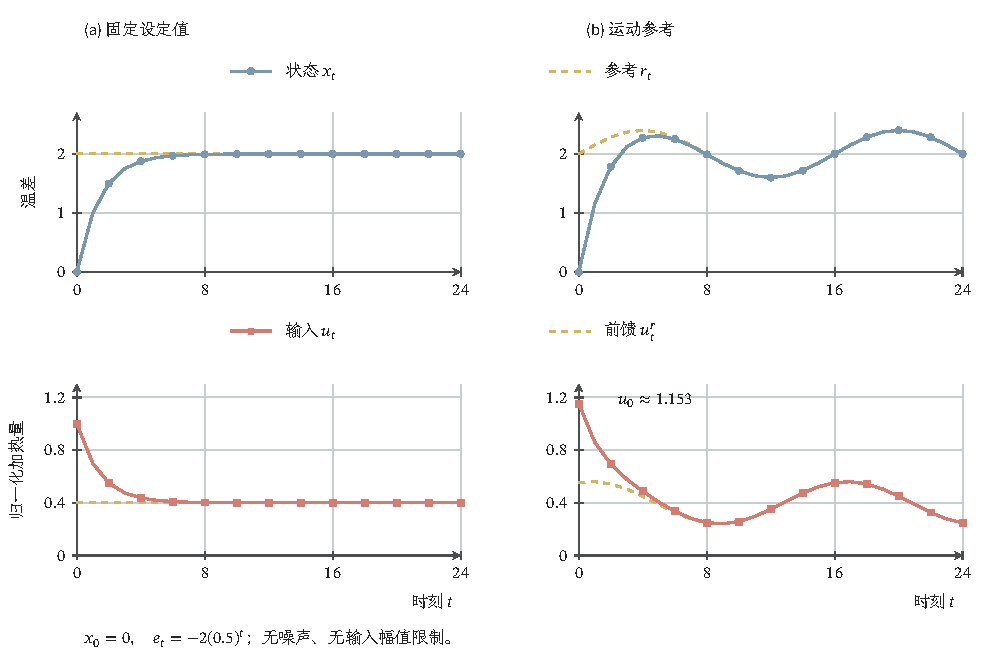
\includegraphics[width=\linewidth]{figures/01-mathematical-preliminaries/05-dynamical-systems-control-decision-and-games/tikz/control/temperature-regulation-tracking.pdf}
  \caption{同一无噪声温度模型、初态$x_0=0$与误差增益$0.3$下的调节和跟踪。
  左列固定$r_t=2$，右列取$r_t=2+0.4\sin(\pi t/8)$；上排比较参考与实际状态，
  下排比较维持参考的前馈与完整输入。两种任务的误差均为$e_t=-2(0.5)^t$，
  但运动参考需要持续变化的前馈。图中输入无幅值限制，右下首个动作超过$1$，
  因而此图不是受限执行器的安全证明。离散点之间连线仅便于阅读。}
  \label{fig:control-temperature-regulation-tracking}
\end{figure*}

误差趋零、误差有界与始终不超过某阈值仍有区别。
无扰动时，$|e_t|=0.5^t|e_0|$既给出收敛，也给出从首步起的范围；
一般多维稳定矩阵可能先放大误差，需要使用$M\rho^t$而不能省掉$M$。
只证明$\sup_t\|\bm e_t\|<\infty$不说明误差是否足够小。
参考位于安全集内也不保证实际状态安全，必须把参考与误差范围相加后再核对约束。

\subsubsection{扰动与模型偏差下的轨迹跟踪}
真实动态与参考规划常有偏差。设实际系统为
$\bm x_{t+1}=(\bm A+\Delta\bm A)\bm x_t+
(\bm B+\Delta\bm B)\bm u_t+\bm d_t$，
名义参考的实现残差为
$\bm\eta_t=\bm A\bm r_t+\bm B\bm u_t^r-\bm r_{t+1}$。
沿用名义前馈加反馈后，误差的完整方程为
\begin{equation}
  \begin{aligned}
  \bm e_{t+1}
  ={}&(\bm F+\Delta\bm A-\Delta\bm B\bm K)\bm e_t\\
     &+\Delta\bm A\bm r_t+\Delta\bm B\bm u_t^r+\bm\eta_t+\bm d_t,
  \qquad \bm F=\bm A-\bm B\bm K.
  \end{aligned}
  \label{eq:control-tracking-model-error}
\end{equation}
偏差既改变误差反馈矩阵，也使原先可实现的参考变成受迫误差来源。
因此只验证名义$\bm F$稳定，还不足以覆盖任意模型误差。

固定一种向量范数及相容矩阵范数，假设$\|\bm F\|\leq\rho<1$，
$\|\Delta\bm A-\Delta\bm B\bm K\|\leq\varepsilon$且
$q:=\rho+\varepsilon<1$。稳定矩阵可以在适当范数中取得收缩界，
但偏差界和以下所有大小必须在同一范数下计算，不能混用欧氏范数数值。
若$\|\bm r_t\|\leq R_0,\|\bm u_t^r\|\leq U_0$，
且$\|\bm\eta_t\|\leq\bar\eta,\|\bm d_t\|\leq\bar d$，令
$D=\|\Delta\bm A\|R_0+\|\Delta\bm B\|U_0+\bar\eta+\bar d$，则
\begin{equation}
  \|\bm e_t\|\leq q^t\|\bm e_0\|
         +\frac{1-q^t}{1-q}D.
  \label{eq:control-tracking-error-bound}
\end{equation}
证明只需由式~\eqref{eq:control-tracking-model-error}取范数，
再展开$\|\bm e_{t+1}\|\leq q\|\bm e_t\|+D$的几何级数。
若受迫项趋零且齐次误差仍稳定，误差也趋零；若受迫项仅有界，
一般只能保证$\limsup_t\|\bm e_t\|\leq D/(1-q)$。
积分器可消除合适模型下的常值输出偏差，不能无条件抵消任意运动参考产生的时变失配。

在精确温度模型中，若$|d_t|\leq0.1$，
则$|e_t|\leq0.5^t|e_0|+0.2(1-0.5^t)$。
若希望误差始终位于$[-\delta,\delta]$，应检查
$|e_0|\leq\delta$及$0.5\delta+0.1\leq\delta$，
而不只报告最终误差界。对前述正弦参考，选择$\delta=0.6$时，
实际状态落在$[1.0,3.0]$，输入落在约$[0.059,0.741]$；
在这个误差范围内，参考加上误差仍满足状态约束，前馈加上反馈也满足输入
约束。这就给出了跟踪与安全同时成立的一组局部条件。
图中的$e_0=-2$不在这个范围，不能套用这项保证。

如果安全控制器把名义动作改为
$\bm u_t=\bm u_t^r-\bm K\bm e_t+\Delta\bm u_t^{\mathrm s}$，
精确模型的误差方程还多出$\bm B\Delta\bm u_t^{\mathrm s}$。
修正有界时可并入误差界；修正逐渐消失时可恢复无扰动的渐近跟踪。
若目标与安全约束冲突，修正可能始终不消失，此时必须保留安全并承认跟踪目标不可实现，
不能同时宣称两项保证。

\section{策略的约束与安全}
\label{sec:control-safety-cbf}

即使控制器能使误差最终变小，纠偏过程中仍可能越界。现在固定允许状态与输入范围，
把每一步可行的动作连接到整段轨迹的安全性，再用这些条件修正调节或跟踪动作。
安全条件决定能选什么，性能准则决定在其中选哪个；二者须分别验证。

\subsection{状态约束下的安全区域}
一个制动系统最终停下，仍可能在停下之前越过位置边界；平均成本很小的随机系统，
也可能有不可接受的少数路径。安全集合（safe set）直接规定允许出现的状态。
对确定性离散闭环$\bm x_{t+1}=F_\kappa(\bm x_t)$，集合$S$安全保持的条件为
\begin{equation}
  F_\kappa(S)\subseteq S.
  \label{eq:control-discrete-invariance}
\end{equation}
从$\bm x_0\in S$出发，应用一步条件得到$\bm x_1\in S$，
归纳便有所有$\bm x_t\in S$。反之，若要求$S$内每个初态均不离开$S$，
特别考察其第一步，就得到上述包含关系。因此它对确定性离散闭环既充分又必要。

例如$x_{t+1}=x_t+u_t$的安全集合为$[0,\infty)$。
反馈$u_t=-1.5x_t$给$x_{t+1}=-0.5x_t$，虽然幅值趋零，
却使任意$x_0>0$在第一步越界；$u_t=-0.5x_t$给$x_{t+1}=0.5x_t$，
既稳定又保持非负。图~\ref{fig:control-stability-safety}保留这一对照，
应观察整段轨迹，而不只看最终状态。原系统能到达负半轴也只说明可达，
不说明所选闭环应当到达那里。
\begin{figure}[htbp]
  \centering
  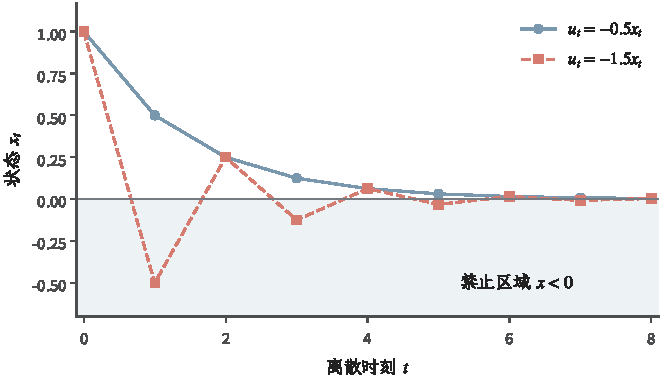
\includegraphics[width=\linewidth]{figures/01-mathematical-preliminaries/05-dynamical-systems-control-decision-and-games/matplotlib/dynamics/stability-safety.pdf}
  \caption{教学系统$x_{t+1}=x_t+u_t$从$x_0=1$出发。
  蓝色圆点采用$u_t=-0.5x_t$，保持$x_t\geq0$；
  红色方点采用$u_t=-1.5x_t$，第一步进入禁止的负半轴后交替衰减。
  两者都渐近稳定，只有前者保持安全集合。灰色区域表示禁止状态。}
  \label{fig:control-stability-safety}
\end{figure}

连续时间还需保证两个观测时刻之间也不越界。考虑控制仿射系统
\begin{equation}
  \dot{\bm x}_t=\bm f(\bm x_t)+\bm G(\bm x_t)\bm u_t,
  \qquad \bm u_t\in U,
  \label{eq:control-affine-system}
\end{equation}
其中$\bm x_t\in\mathbb R^n,\bm u_t\in\mathbb R^m$，
$\bm G(\bm x)\in\mathbb R^{n\times m}$。假设$\bm f,\bm G$局部Lipschitz，
且所选反馈给出存在且唯一的闭环解。以$C^1$函数$h$表示安全集合
\begin{equation}
  S=\{\bm x:h(\bm x)\geq0\}.
  \label{eq:control-safe-set}
\end{equation}
\begin{definition}[正向不变集]
\label{def:control-forward-invariance}
若任意$\bm x_0\in S$所产生的闭环解，在其存在的全部未来时刻均位于$S$，
称$S$对该闭环正向不变（forward invariant）。
\end{definition}
这是定义~\ref{def:dynamical-invariant-limit-sets}在可选择输入的系统中的应用：
本节需要设计使集合保持不变的反馈，而不是只分析已给定规律。
若要说“所有$t\geq0$”，还必须排除有限时间解爆破。

若边界$\partial S=\{h=0\}$光滑且其上$\nabla h\neq\bm0$，
内侧对应$h$增大的方向。Nagumo边界条件要求闭环速度指向内侧或与边界相切：
\begin{equation}
  \nabla h(\bm x)^\top
  [\bm f(\bm x)+\bm G(\bm x)\bm u]\geq0
  \quad\text{当 }h(\bm x)=0.
  \label{eq:control-nagumo-boundary}
\end{equation}
在闭集、正则边界和适定闭环等条件下，它给出正向不变判据。
边界梯度退化时不能机械沿用这条光滑表达，应检查真实切锥。
控制器还需要在接近边界时就限制动作，下面把边界条件扩展到集合附近。

\subsection{安全条件下的可行动作}
函数$h$只用符号区分安全与否，不必等于几何距离。
动作是否安全取决于$h$沿速度的变化，链式法则给出
\[
  L_{\bm f}h(\bm x)=\nabla h(\bm x)^\top\bm f(\bm x),
  \qquad
  L_{\bm G}h(\bm x)=\nabla h(\bm x)^\top\bm G(\bm x).
\]
它们称为\term{Lie导数}（Lie derivative），分别表示无控制漂移与控制方向对
安全函数变化率的贡献。本章的扩展类$\mathcal K$函数指连续、严格递增、
局部Lipschitz且$\alpha(0)=0$的$\alpha:\mathbb R\to\mathbb R$；
例如$\alpha(r)=\gamma r,\gamma>0$。局部Lipschitz条件用于标量比较系统的唯一性。

在安全区域内部，控制器可以允许$h$减小，使状态接近边界，但要限制减小速度；
到达边界$h=0$时，则必须禁止$h$继续减小。下式用$-\alpha(h)$同时表达这两项要求。
\begin{definition}[零化控制屏障函数]
\label{def:control-cbf}
若在包含$S$的开区域$D$中，每个状态都存在$\bm u\in U$使
$L_{\bm f}h(\bm x)+L_{\bm G}h(\bm x)\bm u\geq-\alpha(h(\bm x))$，
则称$h$为该区域上的零化控制屏障函数（control barrier function, CBF）。
其上确界表达为
\begin{equation}
  \sup_{\bm u\in U}
  \{L_{\bm f}h(\bm x)+L_{\bm G}h(\bm x)\bm u\}
  \geq-\alpha(h(\bm x)),
  \label{eq:control-cbf-existence}
\end{equation}
并要求有实际动作满足该阈值；特别是上确界恰等于阈值时，必须能够取到。
\end{definition}
CBF把“留在区域内”变成每个状态可检查的动作不等式。
当$U$紧且动作函数连续时，上确界可取到，数值不等式就足够；
对非紧$U$，若上确界严格大于阈值，也能选到满足阈值的动作，
不必要求无穷大的上确界被取到。真正需要的是以下集合非空：
\begin{equation}
  K_{\mathrm{cbf}}(\bm x)=
  \{\bm u\in U:L_{\bm f}h(\bm x)+L_{\bm G}h(\bm x)\bm u
                      \geq-\alpha(h(\bm x))\}.
  \label{eq:control-cbf-action-set}
\end{equation}
执行器约束已经通过$\bm u\in U$取交集，不能先忽略输入上限设计动作，
再默认饱和后的动作仍符合屏障条件\scite{math-ames2017cbf}

\begin{theorem}[CBF条件保证正向不变]
\label{thm:control-cbf-invariance}
设式~\eqref{eq:control-affine-system}及安全函数满足上述正则条件。
若反馈$\bm u=\kappa(\bm x)$局部Lipschitz，并在包含$S$的开区域$D$中始终满足
$\kappa(\bm x)\in K_{\mathrm{cbf}}(\bm x)$，
则$S$在相应闭环解存在的时间区间内正向不变。
\end{theorem}
\begin{proof}
沿任意闭环解记$r_t=h(\bm x_t)$，链式法则和CBF约束给出
$\dot r_t\geq-\alpha(r_t)$。考虑比较系统
\[
  \dot z_t=-\alpha(z_t),\qquad z_0=r_0\geq0.
\]
$\alpha$局部Lipschitz，比较系统局部解唯一，且$z=0$是平衡解；
从非负初值出发的解不能穿过零点。又因$\alpha$严格递增且$\alpha(0)=0$，
$z_t$留在$[0,z_0]$内，所以比较解在任意有限时间存在。
为验证微分不等式中的$r_t$也不低于$z_t$，在轨迹位于$D$的任一紧时间区间上，
取$\alpha$在两条标量轨迹值域所在紧区间的Lipschitz常数$L$，并令
$q_t=\max\{z_t-r_t,0\}$。在$z_t>r_t$处，
\[
 \dot q_t=\dot z_t-\dot r_t
 \leq-\alpha(z_t)+\alpha(r_t)\leq Lq_t.
\]
正部函数绝对连续，且在其零集上导数几乎处处为零，故这个不等式几乎处处成立。
由$q_0=0$可得$q_t\leq L\int_0^tq_s\,\mathrm ds$；
引理~\ref{lem:action-state-gronwall}遂给出$q_t=0$，即$r_t\geq z_t\geq0$。
因为$D$是包含$S$的开区域，若轨迹离开$S$，必先在$D$中穿过$h=0$进入$h<0$，
与比较不等式矛盾。故在闭环解存在的全部时间内，$\bm x_t\in S$。

对$\alpha(r)=\gamma r$还可以直接验证：
\[
  \frac{\mathrm d}{\mathrm dt}(e^{\gamma t}r_t)
  =e^{\gamma t}(\dot r_t+\gamma r_t)\geq0.
\]
所以$r_t\geq e^{-\gamma t}r_0\geq0$。
当$r=0$时约束退化为$\dot r\geq0$，与边界条件一致。
\end{proof}
这项证明依赖动作约束始终可行、反馈与动态足够规则，以及动作按连续时间模型实际施加。
某一个采样点的动作朝内，不能代替这些沿轨迹的条件。

回到离散温度系统，令$S=[0,3],U=[0,1]$且无噪声。
下一步安全要求$0\leq0.8x+u\leq3$，因此精确的一步安全动作集合为
\begin{equation}
  K_{\mathrm{safe}}(x)
  =[\,\max\{0,-0.8x\},\ \min\{1,3-0.8x\}\,].
  \label{eq:control-temperature-safe-actions}
\end{equation}
对$x\in[0,3]$，下端为$0$，上端至少为$0.6$，所以每个安全状态都有可行动作。
固定目标反馈$u=0.4-0.3(x-2)=1-0.3x$在该区间取值于$[0.1,1]$，
下一状态为$1+0.5x\in[1,2.5]$。它不需要修正就同时实现输入可行、状态安全与趋于$2$。
这个显式包含关系比“反馈稳定”多证明了整个区间的安全保持。

\subsection{可行约束下的反馈修正}
若调节或跟踪给出的名义动作$\bm u_{\mathrm{nom}}$不可行，
可以在每个状态寻找对它修改最小的安全动作：
\begin{equation}
  \begin{aligned}
  \bm u^\ast(\bm x)\in\argmin_{\bm u\in U}\quad&
    \tfrac12(\bm u-\bm u_{\mathrm{nom}})^\top
              \bm H(\bm u-\bm u_{\mathrm{nom}})\\
  \text{s.t.}\quad&
    L_{\bm f}h(\bm x)+L_{\bm G}h(\bm x)\bm u
       \geq-\alpha(h(\bm x)),
  \end{aligned}
  \label{eq:control-cbf-qp}
\end{equation}
其中$\bm H\succ\bm0$规定修改各输入分量的代价。
CBF约束对输入线性；$U$为多面体时这是二次规划（quadratic program, QP），
一般非空闭凸$U$则给出闭凸约束下的二次优化问题。
第~\ref{chap:optimization}章的约束优化工具可用于计算它。
目标只比较当前动作的距离，并不使修正后的整条轨迹保持原LQR成本最优。

\begin{example}[一维积分器上的安全投影]
\label{ex:control-cbf-scalar-projection}
考虑$\dot x_t=u_t$、$S=[0,\infty)$、$h(x)=x$及$\alpha(h)=\gamma h$。
CBF条件为$u\geq-\gamma x$。若$U=\mathbb R,H=1$，解为
\begin{equation}
  u^\ast(x)=\max\{u_{\mathrm{nom}}(x),-\gamma x\}.
  \label{eq:control-cbf-scalar-projection}
\end{equation}
在$x=0.2,\gamma=1$且名义动作恒为$u_{\mathrm{nom}}=-1$时，动作修正为$-0.2$。
持续应用该反馈，状态按$x_t=0.2e^{-t}$接近零而不穿过边界。
若执行器另要求$u\leq-0.5$，此处与$u\geq-0.2$冲突，QP不可行；
安全函数的形式本身不能保证执行器能够提供所需动作。
\end{example}

在上述凸约束下，若可行域非空且闭，正定二次目标在动作范数增大时趋于无穷，
所以极小点存在；严格凸性保证动作唯一。没有闭性时，严格凸只说明已有极小点至多一个，
不能保证下确界取到。即使每个状态上的优化问题都有唯一解，从状态到动作的映射$\bm x\mapsto\bm u^\ast(\bm x)$
也未必局部Lipschitz：约束梯度退化、活跃约束切换或可行域突变可能破坏正则性。
应用不变性定理前，还需按约束资格条件与参数化优化结果核验反馈的规则性。

\begin{example}[圆形障碍外的安全修正]
\label{ex:control-cbf-obstacle}
对平面单积分器$\dot{\bm p}_t=\bm u_t$，
障碍中心为$\bm c$、半径为$r>0$。取
$h(\bm p)=\|\bm p-\bm c\|_2^2-r^2$，安全区域是圆外。
$\alpha(h)=\gamma h$给出
\begin{equation}
  2(\bm p-\bm c)^\top\bm u
  \geq-\gamma(\|\bm p-\bm c\|_2^2-r^2).
  \label{eq:control-cbf-obstacle-constraint}
\end{equation}
在边界$\bm p-\bm c=(r,0)^\top$，名义动作$(-v,0)^\top,v>0$指向障碍内部，
左侧为$-2rv<0$。无其他输入约束且$\bm H=\bm I$时，
QP将动作投影到半空间$2(\bm p-\bm c)^\top\bm u\geq0$，
此处修正为$\bm u^\ast=\bm0$。
若名义动作含有切向分量，投影保留切向分量，只移除向内的法向分量。
停在边界是安全的，却未必能够完成绕行任务。
\end{example}

多个$h_i(\bm x)\geq0$会产生多条动作约束。
每条单独可行，不代表它们与执行器限制联合可行；障碍、制动能力或转向限制可能相互冲突。
加入松弛变量使优化器返回数值解，同时也允许原安全条件被违反，
因而不能再声明原来的硬不变性保证。此时应说明约束冲突后怎样处理、在哪些区域还能恢复安全，或改为保证多大的
越界概率；不能继续使用原先的硬安全结论。
图~\ref{fig:control-barrier-projection}用$(x,u)$平面显示一维投影：
每个固定状态的安全动作是一条竖直半直线，修正沿这条半直线寻找最近点。
\begin{figure}[htbp]
  \centering
  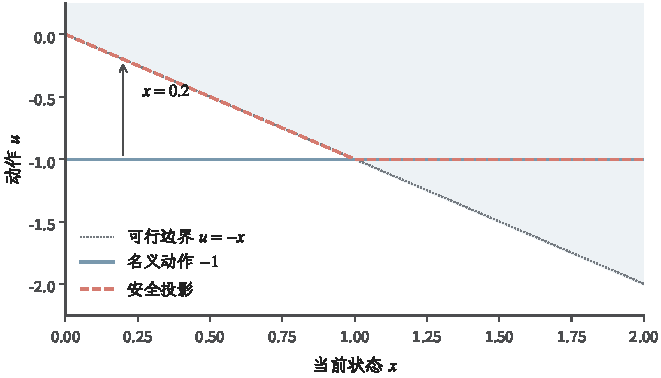
\includegraphics[width=\linewidth]{figures/01-mathematical-preliminaries/05-dynamical-systems-control-decision-and-games/matplotlib/dynamics/barrier-projection.pdf}
  \caption{教学积分器$\dot x_t=u_t$、安全集合$x\geq0$及$\alpha(h)=h$。
  灰色虚线$u=-x$上方为允许动作；蓝色实线为名义动作$u=-1$，
  红色虚线为投影$u^\ast=\max\{-1,-x\}$。
  $x\geq1$处无需修正，$x=0.2$处修正为$-0.2$。
  图中没有额外执行器限制，不能据此判断有限输入范围下的联合可行性。}
  \label{fig:control-barrier-projection}
\end{figure}
\FloatBarrier

对温度模型，使用式~\eqref{eq:control-temperature-safe-actions}的闭区间投影：
\[
  u_t=\min\{u_{\max}(x_t),\max\{u_{\min}(x_t),u_{\mathrm{nom},t}\}\}.
\]
前述正弦跟踪从$x_0=0$出发，名义首个动作为
$0.4+0.4\sin(\pi/8)+0.6\approx1.153$，投影改为$u_0=1$。
于是$x_1=1$，而不是无约束的$1.153$；此时
$e_1=1-[2+0.4\sin(\pi/8)]\approx-1.153$，不再等于$0.5e_0=-1$。
由于每步安全动作集合非空，重复投影仍保持$0\leq x_t\leq3$及$0\leq u_t\leq1$，
但跟踪误差须按增加了修正项的方程重新分析。
目标参考持续要求超出能力的输入时，不能同时保持精确跟踪；
安全投影的“最近”也不等于全时域最优。

\subsection{扰动与离散执行下的安全保证}
若真实连续动态含$\|\bm d_t\|_2\leq\delta$的加性扰动，
最坏方向使安全函数的导数减少至多$\|\nabla h(\bm x)\|_2\delta$。
因此鲁棒充分条件为
\begin{equation}
  L_{\bm f}h+L_{\bm G}h\,\bm u
  \geq-\alpha(h)+\|\nabla h\|_2\delta.
  \label{eq:control-robust-cbf}
\end{equation}
有有效上界的模型误差可并入同一裕量。没有经过验证的误差界时，
任意加一个“安全系数”只是经验缓冲，不能推出鲁棒正向不变性。

离散温度系统若$|w_{t+1}|\leq\delta$，最坏扰动下的安全动作集合为
\begin{equation}
  K_{\mathrm{safe}}^\delta(x)
  =[\,\max\{0,\delta-0.8x\},\
       \min\{1,3-\delta-0.8x\}\,].
  \label{eq:control-temperature-robust-actions}
\end{equation}
当$0\leq\delta\leq0.6$，该集合对所有$x\in[0,3]$非空：
下端不超过$1$，未截断区间宽度$3-2\delta$非负，且上端在$x=3$也不小于零。
若$\delta>0.6$，从$x=3$面对正向最大扰动，即使取最小输入$u=0$也会越界，
所以整个$[0,3]$不能在这类扰动下保持不变。
固定目标的名义反馈产生$1+0.5x+w_{t+1}$，对$\delta\leq0.5$已经落在$[0,3]$，
因而无需修正。高斯噪声没有有限的确定幅值界，不能套用这个逐路径保证；
概率风险要按第~\ref{chap:decision-theory-and-dynamic-risk}章的风险口径另行定义。

数字控制器每隔$\Delta$更新动作，并在区间内保持不变。
采样点满足连续CBF约束，不自动保证区间内部满足，因为状态和安全导数仍在变化。
例如对固定保持动作，若
$g(\bm x,\bm u)=L_{\bm f}h+L_{\bm G}h\,\bm u+\alpha(h)$
在已核验区域内对状态的Lipschitz常数为$L_g$，且速度有界$\|\dot{\bm x}\|\leq M$，
则区间内$g$最多降低$L_gM\Delta$。
采样时预留这一裕量才可保证区间内$g\geq0$；区域与速度界本身也须有效，
不能假定在尚未证明安全的区域外仍成立。

也可以直接构造离散屏障条件
\[
  h(\bm x_{t+1})-h(\bm x_t)\geq-\alpha_{\mathrm d}(h(\bm x_t)),
\]
并要求每个$r\geq0$都有$0\leq\alpha_{\mathrm d}(r)\leq r$。
这样$h(\bm x_t)\geq0$便推出
$h(\bm x_{t+1})\geq h(\bm x_t)-\alpha_{\mathrm d}(h(\bm x_t))\geq0$，
可逐步归纳安全性。常用$\alpha_{\mathrm d}(r)=\gamma r$取$0<\gamma\leq1$。
若离散模型只是连续系统的采样映射，采样点安全仍不等于区间安全，
还需检查采样间轨迹；在预测时域中直接验证整段连续轨迹是另一种办法。

还有一种限制来自\term{相对阶}（relative degree），即对某个输出求导多少次，
当前输入才第一次显式出现。若$L_{\bm G}h=\bm0$，一阶CBF约束不含动作。
例如双积分器$\dot p_t=v_t,\dot v_t=u_t$用
$h(p)=p-p_{\min}$保护位置下界，有$\dot h=v$、$\ddot h=u$，
因此相对阶为$2$。此时需要递归控制更高导数，或把速度与制动距离纳入安全函数。
取$\psi_1=v+k_1h$（$k_1>0$），若再约束
\[
  u+k_1v+k_2\psi_1\geq0,\qquad k_2>0,
\]
则$\dot\psi_1\geq-k_2\psi_1$。在初态同时满足$h\geq0,\psi_1\geq0$、
约束始终可行且闭环适定时，比较原理先保证$\psi_1\geq0$，
再由$\dot h\geq-k_1h$保证$h\geq0$。
新增的速度条件不可省略，执行器幅值也可能使这条高阶约束不可行。

例如$p-p_{\min}=0.1,v=-1$，最大制动加速度为$2$，
最快停止距离$v^2/(2u_{\max})=0.25$已超过剩余距离。
此时位置虽在允许区间，任何允许动作也不能避免后续越界。
安全初态应同时考虑位置与速度；把一阶公式套到$L_{\bm G}h=0$处，
只会得到与输入无关的条件。

CBF还要求用于计算约束的状态信息可靠。
若只有估计值，应先给估计误差集合界或概率模型，再收紧安全集合或构造输出反馈屏障。
把估计均值直接当作真实状态代入，只能验证估计轨迹，
不能从有界误差协方差自动推出真实轨迹的硬安全。

\section{本章小结}
\label{sec:control-theory-summary}

一个可实施策略既要遵守信息时序，也要符合执行器能够改变的方向。
可控、可观测要求处理全部状态方向；可稳定要求输入无法影响的模式已经稳定，可检测要求观测无法区分的误差
模式能够自行衰减。
它们为设计提供结构条件，真正的轨迹行为仍由闭环矩阵、误差动态或Lyapunov不等式决定。
增益还会改变输入幅值和中间阶段的响应，所以不同稳定反馈并非可以不加区别地互换。

在同一温度模型中，固定目标$2$需要平衡输入$0.4$，
再加本章选取的误差反馈，才得到$e_{t+1}=0.5e_t$。
运动参考改用$u_t^r=r_{t+1}-0.8r_t$抵消参考变化，
同一个稳定误差系统便能服务于跟踪。常值扰动、时变扰动和模型偏差改变这一结论：
合适的积分增广可以消除常值输出偏差，对一般的持续扰动，通常只能给出误差范围，
非零随机噪声则应区分均值收敛、协方差有界与路径收敛。

Riccati方法在特定二次成本下选择反馈。有限时域的逐步配方保持二次形式；
确定性无折扣无限时域还需可稳定、成本可检测及权重条件，
才能同时得到稳定化与成本最优性。输出反馈通过估计连接实际信息，
确定性系统中分开设计反馈与观测器的谱结论，以及随机系统中的稳态误差
结论，各有适用条件，
不能把它们推广成任意观测、约束或模型失配下的保证。

安全性约束全过程。对无噪声温度系统，固定目标反馈已经保持
$0\leq u\leq1,0\leq x\leq3$；同一增益的运动参考却可能在初始纠偏时要求过大输入。
一步安全集合或连续屏障约束可以修正动作，但修正后的调节、跟踪与价值必须重新核验。
约束不可行、扰动无有效上界、采样间行为未检查或状态估计不可靠时，
都不能沿用名义安全结论。
第~\ref{chap:decision-theory-and-dynamic-risk}章将进一步比较这些策略的
累计成本、收益与风险；目标可达、误差收敛、轨迹安全和价值最优仍是需要分别回答的问题。
